\section{Results}\label{sec:results}

This chapter compares the performance of rule-based trade classification against machine learning-based classification. 

\subsection{Results of Rule-Based Approaches}\label{sec:result-of-rule-based-approaches}

We estimate the accuracy of classical trade classification rules on the \gls{ISE} and \gls{CBOE} samples. We consider the tick and quote rule, as well as the \gls{LR} algorithm, \gls{EMO} rule, and \gls{CLNV} method in their classical and reversed formulation. Additionally, we consider the \gls{GSU} method (small) and \gls{GSU} method (large) due to their state-of-the-art performance on the validation set, as derived in \cref{sec:hyperparameter-tuning}.

We report in \cref{tab:ise-classical} accuracies for the entire data set and separate subsets spanning the periods of train, validation, and test set as defined in \cref{sec:train-test-split}. Doing so enables comparisons with previous works, but also provides meaningful estimates on the test set relevant for benchmarking purposes. Our results are approximately similar to \textcite[\checkmark][40--42]{grauerOptionTradeClassification2022}. Minor deviations exist, which can be pinned down to differences in handling of unclassified trades and non-positive spreads, as well as divergent implementations of the depth rule.\footnote{Correspondence with the author.}

From all rules, the tick rule performs worst when applied to trade prices at the trading venue with accuracies of a random guess, \SI{49.67}{\percent}. For comparison, a simple majority vote achieves \SI{51.40}{\percent} accuracy. The tick test performs best when estimated on the consecutive trade prices, and additionally, when estimated at the inter-exchange level marginally improves over a random classification, achieving accuracies of \SI{55.25}{\percent} for the reversed tick test. Due to the poor performance, of tick-based algorithms at the exchange level, we estimate all hybrids with last/next differing price from any exchange, distinguished by $\operatorname{tick}_{\mathrm{all}}$ or $\operatorname{rtick}_{\mathrm{all}}$.

Quote-based algorithms outperform tick-based algorithms delivering accuracy up to \SI{63.72}{\percent} when estimated on the \gls{NBBO}. The superiority of quote-based algorithms in option trade classification has previously been documented in \textcites[\checkmark][891]{savickasInferringDirectionOption2003}[\checkmark][3]{grauerOptionTradeClassification2022}.

\begin{table}[ht]
    \centering
    \caption[Accuracies of Rule-Based Approaches on \glsentryshort{ISE}]{This table shows the accuracy of common trade classification rules and their variations for option trades on \gls{ISE} sample. Unclassifiable trades by the respective rule are assigned randomly as buy or sell. Hybrid methods are estimated using trade prices across all exchanges. We report the percentage of classifiable trades and the overall accuracy for subsets based on our train-test split and the entire dataset. The best rule is in bold.}
    \label{tab:ise-classical}
    \begin{tabular}{@{}lSSSSS@{}}
        \toprule
        {}                                     & {Coverage in \%}  & \multicolumn{4}{c}{Accuracy in \%}                                                             \\ \cmidrule(lr){2-2} \cmidrule(lr){3-6}
        {Classification Rule}                  & {All}             & {Train}                            & {Val}             & {Test}            & {All}             \\\midrule
        $\operatorname{tick}_{\mathrm{ex}}$    & 91.5794           & 49.1842                            & 50.5441           & 50.2394           & 49.6674           \\
        $\operatorname{rtick}_{\mathrm{ex}}$   & 90.3529           & 52.1701                            & 50.3068           & 50.5258           & 51.4682           \\
        $\operatorname{quote}_{\mathrm{ex}}$   & 91.1158           & 66.2807                            & 57.5355           & 57.0079           & 62.6747           \\
        $\operatorname{lr}_{\mathrm{ex}}$      & 99.8020           & 66.0269                            & 57.6103           & 57.1019           & 62.5564           \\
        $\operatorname{rlr}_{\mathrm{ex}}$     & 99.6690           & 66.3908                            & 57.7091           & 57.2014           & 62.8143           \\
        $\operatorname{emo}_{\mathrm{ex}}$     & 98.7285           & 56.5416                            & 53.7133           & 53.7864           & 55.4243           \\
        $\operatorname{remo}_{\mathrm{ex}}$    & 98.2749           & 57.1490                            & 53.6360           & 54.1495           & 55.8459           \\
        $\operatorname{clnv}_{\mathrm{ex}}$    & 98.9537           & 60.1181                            & 55.2305           & 54.7502           & 58.0656           \\
        $\operatorname{rclnv}_{\mathrm{ex}}$   & 98.6967           & 60.8498                            & 55.3888           & 55.0784           & 58.6019           \\ \midrule
        $\operatorname{tick}_{\mathrm{all}}$   & 97.8543           & 52.8954                            & 54.5403           & 53.3412           & 53.3134           \\
        $\operatorname{rtick}_{\mathrm{all}}$  & 96.7020           & 55.9539                            & 54.4020           & 53.9891           & 55.2500           \\ \midrule
        $\operatorname{quote}_{\mathrm{nbbo}}$ & 91.7324           & 66.8290                            & 58.5665           & 59.5656           & 63.7223           \\
        $\operatorname{lr}_{\mathrm{nbbo}}$    & 99.8084           & 66.5295                            & 58.6137           & 59.6227           & 63.5635           \\
        $\operatorname{rlr}_{\mathrm{nbbo}}$   & 99.7292           & 66.8227                            & 58.7145           & 59.7062           & 63.7762           \\
        $\operatorname{emo}_{\mathrm{nbbo}}$   & 98.7186           & 58.2850                            & 54.8106           & 55.9278           & 57.1183           \\
        $\operatorname{remo}_{\mathrm{nbbo}}$  & 98.3939           & 58.9415                            & 54.8198           & 56.2168           & 57.5718           \\
        $\operatorname{clnv}_{\mathrm{nbbo}}$  & 98.8975           & 61.5439                            & 56.3371           & 57.0753           & 59.6079           \\
        $\operatorname{rclnv}_{\mathrm{nbbo}}$ & 98.7000           & 62.2628                            & 56.5928           & 57.4307           & 60.1614           \\ \midrule
        $\operatorname{gsu}_{\mathrm{small}}$  & 99.7918           & 66.8171                            & 58.9378           & 60.0508           & 63.8865           \\
        $\operatorname{gsu}_{\mathrm{large}}$  & \bfseries 99.9943 & \bfseries 80.1647                  & \bfseries 69.3726 & \bfseries 67.6112 & \bfseries 75.4922 \\
        \bottomrule
    \end{tabular}
\end{table}

\todo{Better embed with savickas. What did they find for LR algorithm etc. how is their coverage?}

The performance of hybrids, such as the \gls{LR} algorithm, hinges on the reliance on the tick test. Thus, the \gls{EMO} rules and to a lesser extent the \gls{CLNV} rules perform worst, achieving accuracies between \SI{55.42}{\percent} and \SI{57.57}{\percent}. In turn, variants of the \gls{LR}, which uses the quote rule for most trades, are among the best-performing algorithms. By extension, \gls{GSU} method (small) further reduces the dependence on tick-based methods through the successive applications of quote rules, here $\operatorname{quote}_{\mathrm{nbbo}} \to \operatorname{quote}_{\mathrm{ex}}$.

Notably, the \gls{GSU} method (large) featuring overrides from the trade size and depth rules performs best, achieving \SI{67.61}{\percent} accuracy on the test set and \SI{75.49}{\percent} on the entire dataset. Yet, the performance deteriorates most sharply between sets, as visualized in \cref{fig:classical-accuracies-over-time}.

\begin{figure}[ht]
    \centering
    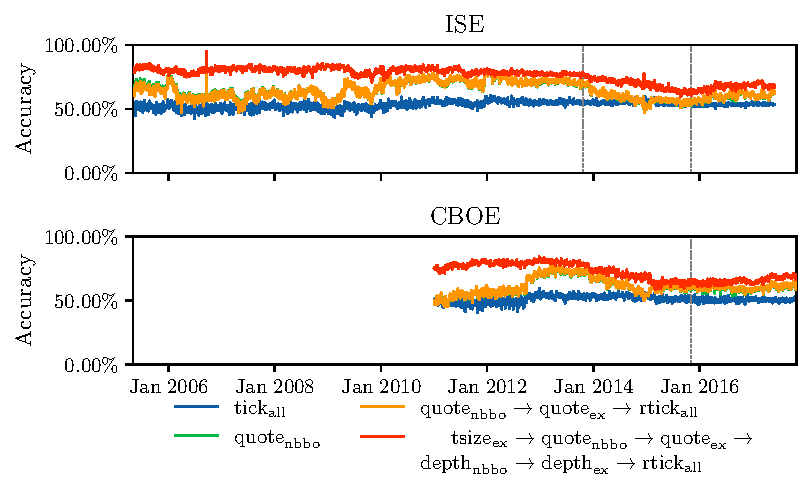
\includegraphics{classical-accuracies-over-time.pdf}
    \caption[Accuracy of Rule-Based Classifiers Over Time]{Accuracy of rule-based classifiers on \gls{ISE} and \gls{CBOE} sample over time. The bar \myline{} indicates the beginning of a new subset based on the train-test split.}
    \label{fig:classical-accuracies-over-time}
\end{figure}

\begin{table}[ht]
    \centering
    \caption[Accuracies of Rule-Based Approaches on \glsentryshort{CBOE}]{This table shows the accuracy of common trade classification rules and their variations for option trades on \gls{CBOE} sample. Unclassifiable trades by the respective rule are assigned randomly as buy or sell. Hybrid methods are estimated using trade prices across all exchanges. We report the percentage of classifiable trades and the overall accuracy for subsets based on our train-test split and the entire dataset. The best rule is in bold.}
    \label{tab:cboe-classical}
    \begin{tabular}{lSSSS}
        \toprule
        {}                                     & {Coverage in \%}  & \multicolumn{3}{c}{Accuracy in \%}                                         \\ \cmidrule(lr){2-2}\cmidrule(lr){3-5}
        {Classification Rule}                  & {All}             & {Pre-Test}                         & {Test}            & {All}             \\\midrule
        $\operatorname{tick}_{\mathrm{ex}}$    & 91.4507           & 48.6156                            & 48.9969           & 48.7469           \\
        $\operatorname{rtick}_{\mathrm{ex}}$   & 90.2769           & 51.0857                            & 50.5432           & 50.8989           \\
        $\operatorname{quote}_{\mathrm{ex}}$   & 90.5150           & 62.6661                            & 62.0689           & 62.4605           \\
        $\operatorname{lr}_{\mathrm{ex}}$      & 99.7455           & 62.3106                            & 61.5831           & 62.0602           \\
        $\operatorname{rlr}_{\mathrm{ex}}$     & 99.4584           & 62.7035                            & 61.9898           & 62.4578           \\
        $\operatorname{emo}_{\mathrm{ex}}$     & 97.9601           & 49.3923                            & 48.6489           & 49.1364           \\
        $\operatorname{remo}_{\mathrm{ex}}$    & 97.3242           & 49.8883                            & 49.9529           & 49.9105           \\
        $\operatorname{clnv}_{\mathrm{ex}}$    & 98.4350           & 54.2644                            & 53.2492           & 53.9149           \\
        $\operatorname{rclnv}_{\mathrm{ex}}$   & 98.0358           & 55.1506                            & 54.5686           & 54.9502           \\\midrule
        $\operatorname{tick}_{\mathrm{all}}$   & 97.2135           & 51.4199                            & 50.4403           & 51.0827           \\
        $\operatorname{rtick}_{\mathrm{all}}$  & 96.0292           & 54.2521                            & 52.7056           & 53.7197           \\\midrule
        $\operatorname{quote}_{\mathrm{nbbo}}$ & 91.1772           & 61.3222                            & 59.8123           & 60.8024           \\
        $\operatorname{lr}_{\mathrm{nbbo}}$    & 99.7705           & 60.9503                            & 59.3730           & 60.4073           \\
        $\operatorname{rlr}_{\mathrm{nbbo}}$   & 99.6335           & 61.3095                            & 59.7608           & 60.7764           \\
        $\operatorname{emo}_{\mathrm{nbbo}}$   & 98.7186           & 51.6420                            & 51.6299           & 51.6378           \\
        $\operatorname{remo}_{\mathrm{nbbo}}$  & 98.3939           & 52.4847                            & 53.0736           & 52.6874           \\
        $\operatorname{clnv}_{\mathrm{nbbo}}$  & 98.8975           & 55.3058                            & 54.1294           & 54.9008           \\
        $\operatorname{rclnv}_{\mathrm{nbbo}}$ & 98.7000           & 56.3217                            & 55.4032           & 56.0055           \\\midrule
        $\operatorname{gsu}_{\mathrm{small}}$  & 99.7918           & 61.8938                            & 60.7464           & 61.4988           \\
        $\operatorname{gsu}_{\mathrm{large}}$  & \bfseries 99.9943 & \bfseries 74.6511                  & \bfseries 66.5176 & \bfseries 71.8510 \\\bottomrule
    \end{tabular}
\end{table}

We repeat the analysis on the \gls{CBOE} dataset in \cref{tab:cboe-classical} and observe a similar ranking to \cref{tab:ise-classical}. Overall, the performance of classical trade classification rules further diminishes or remains at a low level. Tick-based rules trail the performance of quote-based approaches, and the accuracy of hybrids varies with the dependence on the tick test. Different from the \gls{ISE} sample, the quote rule estimated on the \gls{NBBO}, leads to a degraded performance than the quote rule applied to \gls{CBOE} quotes. Again, \gls{GSU} method (small) and \gls{GSU} method (large) perform best, though the strong outperformance does not carry over to the test set as depicted \cref{fig:classical-accuracies-over-time}.\footnote{Performance on \gls{CBOE} can be improved if the order of quote rules is reversed. For full combinatoric coverage see \textcite[\checkmark][44]{grauerOptionTradeClassification2022}. To avoid overfitting the test set by classical rules, we keep the baseline constant following our reasoning from \cref{sec:hyperparameter-tuning}.}

\begin{figure}[!ht]
    \centering
    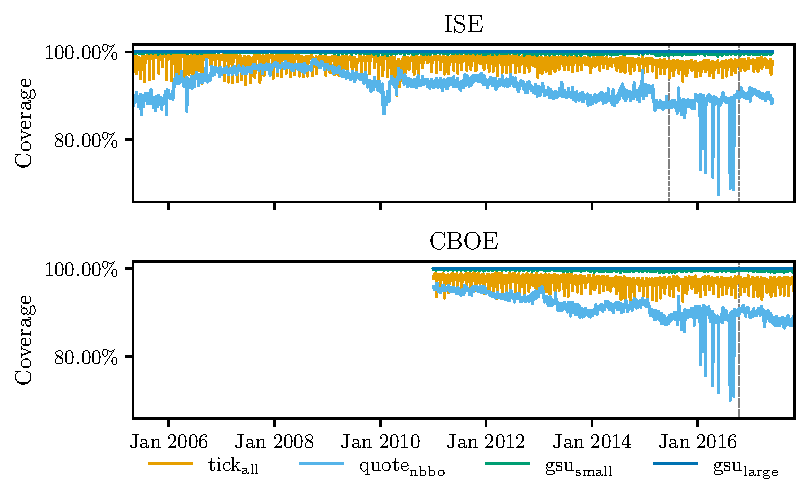
\includegraphics{classical-coverage-over-time.pdf}
    \caption[Coverage of Rule-Based Classifiers Over Time]{Coverage of rule-based classifiers on \gls{ISE} and \gls{CBOE} sample over time. The bar \myline{} indicates the beginning of a new subset based on the train-test split.}
    \label{fig:classical-coverage-over-time}
\end{figure}

From \cref{tab:ise-classical,tab:cboe-classical} we see, that practically all rule-based approaches leave trades unclassified. This is due to conceptual constraints in the rule itself, but also a result of missing or corrupted data, which equally affects rules with theoretical full coverage. As visualized in \cref{fig:classical-coverage-over-time} coverage decreases qualitatively for selected classification rules over time. It is particularly low when the trade initiator is inferred from the \gls{NBBO}. Theoretically, the tick test can achieve full coverage, in our sample it classifies only $\approx$ \SI{91.5}{\percent}, which is significantly lower than coverage rates reported in the stock market \autocite[\checkmark][535]{ellisAccuracyTradeClassification2000}. \todo{how does this compare to option market savickas?} The low, fluctuating coverage stems from the absence of a distinguishable trade price. For the quote rule, we isolate missing or inverted quotes from midspread trades. Through comparison between \cref{fig:classical-coverage-over-time} and \cref{fig:classical-at-mid-over-time} it is evident, that the majority of unclassified trades are midspread trades, whose share increases over time. In our datasets, hybrids, have the advantage of leveraging multiple data sources, resulting in more complete coverage. If, as in the combinations of \textcite[\checkmark][19--20]{grauerOptionTradeClassification2022}, the basic rules are strong individually, higher coverage is associated with better performance, as fewer trades are classified by a fallback mechanism. \todo{How does this explain grauer performance.}
\todo{Describe outliers? How does the number of midspread trades compare?}

\begin{figure}[!ht]
    \centering
    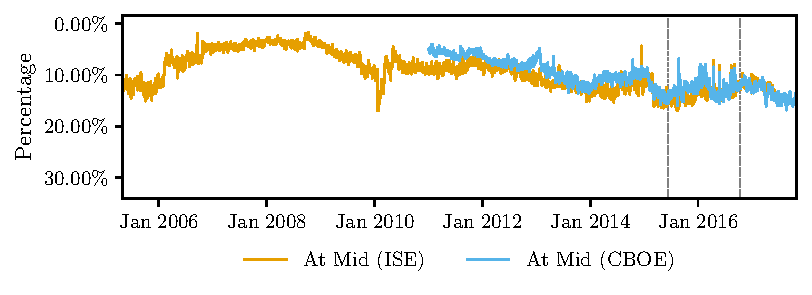
\includegraphics{classical_at_mid_over_time.pdf}
    \caption[Mid-Spread Trades Over Time]{Percentage of midspread trades on \gls{ISE} and \gls{CBOE} sample over time and estimated using \gls{NBBO} quotes. The bar \myline{} indicates the beginning of a new subset based on the train-test split.}
    \label{fig:classical-at-mid-over-time}
\end{figure}

Our machine learning classifiers are robust to missing data, as they can learn alternate patterns for missing features. Next, we test the supervised classifiers on the \gls{ISE}/\gls{CBOE} test sets, which prove to be a challenging test ground for rule-based classifiers as our results from above indicate.

\subsection{Results of Supervised
    Models}\label{sec:results-of-supervised-models}

We test the performance of our supervised models. We take the best configurations from \cref{sec:hyperparameter-tuning}, trained and tuned on the \gls{ISE} trade data, and evaluate their performance on the \gls{ISE} and \gls{CBOE} test sets. \cref{tab:results-supervised-ise-cboe} summarizes the results and benchmarks against state-of-the-art solutions from the literature.

\begin{table}[ht]
    \centering
    \caption[Accuracies of Supervised Approaches]{This table reports the accuracy of supervised \glspl{GBRT} and Transformers for different feature combinations on the \gls{ISE} and \gls{CBOE} datasets. The improvement is estimated as the absolute change in accuracy between the classifier and the benchmark. For feature set classical, $\operatorname{gsu}_{\mathrm{small}}$ is the benchmark and otherwise $\operatorname{gsu}_{\mathrm{large}}$. Models are trained on the \gls{ISE} training set. The best classifier per dataset is in bold.}
    \label{tab:results-supervised-ise-cboe}
    \begin{tabular}{@{}llSSSSSS@{}}
        \toprule
                   &             & \multicolumn{2}{c}{\glsentryshort{FS} Classical} & \multicolumn{2}{c}{\glsentryshort{FS} Size} & \multicolumn{2}{c}{\glsentryshort{FS} Option}                                                                 \\ \cmidrule(lr){3-4}\cmidrule(lr){5-6} \cmidrule(lr){7-8}
        Dataset    & Classifier  & {Acc. in \%}                                     & {+/-}                                                 & {Acc. in \%}                                  & {+/-}              & {Acc. in \%}        & {+/-}              \\ \midrule
        \gls{ISE}  & \gls{GBRT}  & 63.668637                                        & 3.620000                                              & 72.343640                                     & 4.730000           & \bfseries 74.120496 & \bfseries 6.510000 \\
                   & Transformer & \bfseries 63.783020                              & \bfseries 3.730000                                    & \bfseries 72.581107                           & \bfseries 4.970000 & 73.921795           & 6.310000           \\ \addlinespace
        \gls{CBOE} & \gls{GBRT}  & 66.002029                                        & 5.260000                                              & 71.951794                                     & 5.430000           & \bfseries 74.375033 & \bfseries 7.860000 \\
                   & Transformer & \bfseries 66.182348                              & \bfseries 5.440000                                    & \bfseries 72.153338                           & \bfseries 5.640000 & 74.278318           & 7.760000           \\ \bottomrule
    \end{tabular}
\end{table}

Both model architectures consistently outperform their respective benchmarks on the \gls{ISE} and \gls{CBOE} datasets, establishing a state-of-the-art in option trade classification with comparable data requirements. Thereby, Transformers dominate the \gls{ISE} sample when trained on trade prices and quotes reaching \SI{63.783020}{\percent}  in accuracy and \SI{66.18}{\percent} on the \gls{CBOE} sample outperforming previous approaches by \SI{3.730000}{\percent} and \SI{5.440000}{\percent}. Additional trade size features improve the accuracy to \SI{72.581107}{\percent} for the \gls{ISE} sample and \SI{72.153338}{\percent} for the \gls{CBOE} sample. Gradient boosting outperforms all other approaches when trained on additional option features.

While absolute improvements in accuracy over $\operatorname{gsu}_{\mathrm{small}}$ are modest on the smallest feature set, improvements are substantial for larger feature sets ranging between \SI{4.730000}{\percent} to \SI{7.860000}{\percent} over $\operatorname{gsu}_{\mathrm{large}}$. Specifically, the addition of trade size-related features positively contributes to the performance. We discuss feature importances in \cref{sec:feature-importance}.

The results can be enhanced through re-training on the validation set improving accuracies to \SI{76.162269}{\percent}, as documented in \cref{app:results-of-supervised-models-with-re-training}. In favor of conservative estimates, our models in the main text do not use this technique.

To formally test, whether differences between both classifiers are significant, we construct contingency tables and pair-wise compare predictions using McNemar's test \autocite[\checkmark][153--157]{mcnemarNoteSamplingError1947}. We formulate the null hypothesis that both classifiers have the same error rate.
Conceptually similar \textcite[\checkmark][267]{odders-whiteOccurrenceConsequencesInaccurate2000}, uses contingency tables of rule-based methods and true labels. Here, contingency tables are used to pair-wise compare the predictions of \glspl{GBRT} against Transformers.

\begin{table}[!ht]
    \centering
    \sisetup{table-number-alignment=right, table-format=7.0}
    \caption[Contingency Tables of Supervised Classifiers]{This table contains the contingency tables of the supervised classifiers on the \gls{CBOE} and \gls{ISE} test set for feature set classical, classical-size, and option. Cells sum the number of trades, correctly/falsely classified by both classifiers or one. Additionally, McNemar's test statistic $\chi^2$ and the associated $p$-value are reported.}
    \label{tab:contigency-supervised-classifiers}
    \begin{tabular}{@{}llSSSSSS@{}}
        \toprule
                                                                          &           & \multicolumn{2}{c}{{\glsentryshort{FS} Classical}}          & \multicolumn{2}{c}{{\glsentryshort{FS} Size}}      & \multicolumn{2}{c}{{\glsentryshort{FS} Option}}                                             \\
        \cmidrule(l){3-4}\cmidrule(l){5-6}\cmidrule(l){7-8}
        \multicolumn{2}{l}{{$\downarrow$ Trans.$\rightarrow$ \gls{GBRT}}} & {Correct} & {Wrong}                                                     & {Correct}                                                    & {Wrong}                                                     & {Correct} & {Wrong}           \\
        \midrule
        \gls{ISE}                                                         & Correct   & 5904530                                                     & 374201                                                       & 6790958                                                     & 343265    & 6722730 & 586719  \\
                                                                          & Wrong     & 385481                                                      & 3197364                                                      & 366683                                                      & 2360670   & 567124  & 1985003 \\         \addlinespace
                                                                          &           & \multicolumn{2}{l}{{$\chi^2$=\num{167.4593329840644}}}      & \multicolumn{2}{l}{{$\chi^2$=\num{772.3888073492707}}}       & \multicolumn{2}{l}{{$\chi^2$}=\num{332.73576734443077}}                                     \\
                                                                          &           & \multicolumn{2}{l}{{$p$-val.=\num{2.6552012527789754e-38}}} & \multicolumn{2}{l}{{$p$-val.=\num{5.437047807508087e-170}}}  & \multicolumn{2}{l}{{$p$-val.}=\num{2.4374791750246844e-74}}                                 \\
        \midrule
        \gls{CBOE}                                                        & Correct   & 8085066                                                     & 357404                                                       & 8701205                                                     & 502313    & 8746656 & 766824  \\
                                                                          & Wrong     & 380469                                                      & 3968289                                                      & 528093                                                      & 3059617   & 754453  & 2523295 \\         \addlinespace
                                                                          &           & \multicolumn{2}{l}{{$\chi^2$=\num{720.9209389691722}}}      & \multicolumn{2}{l}{{$\chi^2$=\num{644.9465948373747}}}       & \multicolumn{2}{l}{{$\chi^2$=\num{100.58450893558503}}}                                     \\
                                                                          &           & \multicolumn{2}{l}{{$p$-val.=\num{8.441178009879888e-159}}} & \multicolumn{2}{l}{{$p$-val.=\num{2.8062978547775803e-142}}} & \multicolumn{2}{l}{{$p$-val.=\num{1.1345159386344345e-23}}}                                 \\
        \bottomrule
    \end{tabular}
\end{table}

Based on the contingency tables in \cref{tab:contigency-supervised-classifiers}, we observe that both models share a large portion of trades, for which both classifiers agree.\footnote{Through summation of correct classifications of one classifier divided by the matrix sum, one obtains the accuracy from \cref{tab:results-supervised-ise-cboe}. Consider the first entry, e.g., $(\num{5904530}+\num{374201}) / (\num{5904530} + \num{374201} + \num{385481} + \num{3197364}) \approx \num{0.63668637}$.} For larger feature sets, the share of trades correctly classified by one classifier grows, while the number of jointly correctly classified trades plateaus. This can be an indication, that both models learn specific patterns and excel in different trades. The performance differences between classifiers are statistically significant at the \SI{1}{\percent}. The null hypothesis can be rejected.

Relative to related works performing trade classification with machine learning, the improvements are strong, as documented in \cref{app:literature-ml-tc}. As no other work studies the option market or identical model architectures, the results are indicative. The studies report improvements between \SI{1.1}{\percent} and \SI{13.3}{\percent} for their machine learning models over the benchmark. Our absolute improvements exceed all linear models, but the absolute improvements are smaller relative to some tree-based and deep learning models in \textcite[\checkmark][49]{ronenMachineLearningTrade2022}. At the same time, our models are trained on significantly fewer features and on a static training set requiring a fraction of the training cost. We believe, our conservative framing aligns well with scenarios, where trade classification is only a prerequisite to other empirical research.

\todo{check if page 57 isnt the right source of ronen paper.}

Visually, the performance differences between gradient boosting and Transformers on the same feature sets are minor, which is in accordance to \textcites[][]{grinsztajnWhyTreebasedModels2022}[][]{gorishniyRevisitingDeepLearning2021}. These studies conclude, generally for tabular modeling, that neither Transformers nor \glspl{GBRT} are universally superior. Our results validate this observation, specifically for trade classification.
% \todo{It is conceivable, that ...}

% Our findings thereby contradict those of \textcite[][14--49]{ronenMachineLearningTrade2022}, who benchmark tree-based ensembles in the form of random forests and neural networks in the form of \gls{FFN} for trade classification in the equity and bond market and find clear dominance of the tree-based approach. Beyond differences in the market under study and variants, two methodological differences are evident, that explain the diverging results. First, unlike \gls{FFN}, the FT-Transformer is tailored to learn on tabular data through being a rotationally-invariant learner. Second, the data pre-processing and feature engineering is tailored to the requirements of neural networks. Without these measures, tree-based approaches excel due to their robustness in handling skewed and missing data.

Despite the lack of adaption to \gls{CBOE} data, the performance improvements are highest for the \gls{CBOE} dataset. This result is in stark contrast to the of \textcite[\checkmark][32]{ronenMachineLearningTrade2022}, who test random forests for trade classification and report subpar performance. Their setting differs from ours, as they apply ensembles trained in the bond market to equity trades. Moreover, it is unclear if data preprocessing procedures are shared between both sets, which may hamper performance. 

Part of the strong performance on \gls{CBOE} trades hails from weaker benchmark performance, but also from a stronger accuracy of classifiers on the smallest and mid-sized feature sets. One would expect a degradation between sets, assuming exchange-specific trading patterns.

In summary, our supervised methods establish a new state-of-the-art in option trade classification. Our approach achieves full coverage and outperforms all previously reported classification rules in terms of accuracy. Performance transfers across exchanges. We perform additional robustness checks in \cref{sec:robustness-checks} to identify any systematic misclassification.

\subsection{Results of Semi-supervised
    Models}\label{sec:results-of-semi-supervised-models}

We compare the performance of pre-trained Transformers and self-trained gradient-boosting on the \gls{ISE} and \gls{CBOE} test set. Results are reported in \cref{tab:results-semi-supervised-ise-cboe}.

\begin{table}[ht]
    \centering
    \caption[Accuracies of Semi-Supervised Approaches]{This table reports the accuracy of semi-supervised \glspl{GBRT} and Transformers for different feature combinations on the \gls{ISE} and \gls{CBOE} datasets. The improvement is estimated as the absolute change in accuracy between the classifier and the benchmark. For feature set classical, $\operatorname{gsu}_{\mathrm{small}}$ is the benchmark and otherwise $\operatorname{gsu}_{\mathrm{large}}$. Models are trained on the \gls{ISE} training set. The best classifier per dataset is in bold.}
    \label{tab:results-semi-supervised-ise-cboe}
    \begin{tabular}{@{}llSSSSSS@{}}
        \toprule
                   &             & \multicolumn{2}{c}{\glsentryshort{FS} Classical} & \multicolumn{2}{c}{\glsentryshort{FS} Size} & \multicolumn{2}{c}{\glsentryshort{FS} Option}                                                                 \\ \cmidrule(lr){3-4}\cmidrule(lr){5-6} \cmidrule(lr){7-8}
        Dataset    & Classifier  & {Acc. in \%}                                     & {+/-}                                                 & {Acc. in \%}                                  & {+/-}              & {Acc. in \%}        & {+/-}              \\ \midrule
        \gls{ISE}  & \gls{GBRT}  & 63.397514                                        & 3.350000                                              & 72.156489                                     & 4.550000           & 73.536644           & 5.930000           \\
                   & Transformer & \bfseries 64.655751                              & \bfseries 4.600000                                    & \bfseries 72.859054                           & \bfseries 5.250000 & \bfseries 74.551410 & \bfseries 6.940000 \\ \addlinespace
        \gls{CBOE} & \gls{GBRT}  & \bfseries 66.189454                              & \bfseries 5.440000                                    & \bfseries 71.922680                           & \bfseries 5.410000 & 73.953322           & 7.440000           \\
                   & Transformer & 65.668441                                        & 4.920000                                              & 71.783984                                     & 5.270000           & \bfseries 74.095833 & \bfseries 7.580000 \\ \bottomrule
    \end{tabular}
\end{table}

Identical to the supervised case, our models consistently outperform their respective benchmarks. Gradient boosting with self-training surpasses $\operatorname{gsu}_{\mathrm{small}}$ by \SI{3.350000}{\percent} on \gls{ISE} and \SI{5.440000}{\percent} on \gls{CBOE} in accuracy. Improvements for larger feature sets over $\operatorname{gsu}_{\mathrm{large}}$ are marginally lower to the supervised model and range between \SI{4.550000}{\percent} and \SI{7.440000}{\percent}. We already observed a similar result on the validation set in \cref{sec:hyperparameter-tuning}.

Pre-training is beneficial for the performance of Transformers on \gls{ISE} trades, improving over Transformer with random initialization by up to \SI{0.87000}{\percent}. Hence, the performance improvement from pre-training on the validation set carries over the test set. On the \gls{CBOE} dataset, pre-training hurts performance.

\begin{table}[!ht]
    \centering
    \sisetup{table-number-alignment=right, table-format=7.0}
    \caption[Contingency Tables of Semi-Supervised Classifiers]{This table contains the contingency tables of the semi-supervised classifiers on the \gls{CBOE} and \gls{ISE} test set for feature set classical, classical-size, and option. Cells sum the number of trades, correctly/falsely classified by both classifiers or one. Additionally, McNemar's test statistic $\chi^2$ and the associated $p$-value are reported.}
    \label{tab:contigency-semi-supervised-classifiers}
    \begin{tabular}{@{}llSSSSSS@{}}
        \toprule
                                                                          &           & \multicolumn{2}{c}{{\glsentryshort{FS} Classical}}      & \multicolumn{2}{c}{{\glsentryshort{FS} Size}}    & \multicolumn{2}{c}{{\glsentryshort{FS} Option}}                                            \\
        \cmidrule(l){3-4}\cmidrule(l){5-6}\cmidrule(l){7-8}
        \multicolumn{2}{l}{{$\downarrow$ Trans.$\rightarrow$ \gls{GBRT}}} & {Correct} & {Wrong}                                                 & {Correct}                                                  & {Wrong}                                                    & {Correct} & {Wrong}           \\
        \midrule
        \gls{ISE}                                                         & Correct   & 5740391                                                 & 511603                                                     & 6658028                                                    & 457739    & 6665176 & 586696  \\
                                                                          & Wrong     & 635685                                                  & 2973897                                                    & 527023                                                     & 2218786   & 686768  & 1922936 \\         \addlinespace
                                                                          &           & \multicolumn{2}{l}{{$\chi^2$=\num{13419.555125652843}}} & \multicolumn{2}{l}{{$\chi^2$=\num{4874.4103539738535}}}    & \multicolumn{2}{l}{{$\chi^2$}=\num{7863.751971787188}}                                     \\
                                                                          &           & \multicolumn{2}{l}{{$p$-val.=\num{0.0}}}                & \multicolumn{2}{l}{{$p$-val.=\num{0.0}}}                   & \multicolumn{2}{l}{{$p$-val.}=\num{0.0}}                                                   \\
        \midrule
        \gls{CBOE}                                                        & Correct   & 7869540                                                 & 596904                                                     & 8507192                                                    & 692602    & 8634195 & 825343  \\
                                                                          & Wrong     & 530260                                                  & 3794524                                                    & 674861                                                     & 2916573   & 843572  & 2488118 \\         \addlinespace
                                                                          &           & \multicolumn{2}{l}{{$\chi^2$=\num{3940.2335853522645}}} & \multicolumn{2}{l}{{$\chi^2$=\num{230.1397551524246}}}     & \multicolumn{2}{l}{{$\chi^2$=\num{199.0874214684391}}}                                     \\
                                                                          &           & \multicolumn{2}{l}{{$p$-val.=\num{0.0}}}                & \multicolumn{2}{l}{{$p$-val.=\num{5.557306582603872e-52}}} & \multicolumn{2}{l}{{$p$-val.=\num{3.303537049977937e-45}}}                                 \\
        \bottomrule
    \end{tabular}
\end{table}

As evident from \cref{tab:contigency-semi-supervised-classifiers}, a vast majority of trades are classified by both classifiers correctly. For the \gls{ISE}, performance improvements in larger feature sets are driven by trades that are distinctly classified by both classifiers. In turn, at the \gls{CBOE}, the share of common classifications continues to grow. Performance differences between classifiers estimated by the McNemar test are significant.

As no previous work performed semi-supervised classification, we focus our discussion on the performance difference between pre-training and self-training. On \gls{ISE} data, pre-training with the \gls{RTD} objective on unlabeled trades yields significantly stronger performance. The results align with the intuition from \cref{sec:extensions-to-transformer}, that pre-training exposes the model to a larger quantity of trades, which strengthens its ability to learn generalizable knowledge about the data useful in later trade classification. Also, the model is exposed to more diverse trades, as unlabeled trades are not restricted by customer type or trading activity, effectively preventing overfitting.  

An explanation as to why pre-training improves performance on \gls{ISE} but not \gls{CBOE} trades, may be found in the pre-training data and setup. Trades used for pre-training are recorded at the \gls{ISE} only and are repeatedly shown to the model. While our pre-training objective is stochastic with different features being masked in each epoch, past research has shown that repeatedly presenting the same tokens in conjunction with a small-sized pre-training dataset, can degrade performance on the downstream classification task. For instance, \textcite[\checkmark][27--28]{raffelExploringLimitsTransfer2020} document in the context of language modeling that a high degree of repetition encourages memorization in the model, but few repetitions are not harmful. As each trade is only shown $20\times$ to the model, but the size of the dataset is significantly smaller, the true impact remains unclear. Future work could revisit pre-training on a larger subset of LiveVol, incorporating trades from different exchanges, whereby each trade is only shown once to the model. We assume, that such a setup would, analogous to language modeling, improve performance on both \gls{ISE} and \gls{CBOE} trades, as the model is less prone to memorize data and learns a more diverse context.

Self-training with \glspl{GBRT} as a base learner generally performs worse than \glspl{GBRT} trained on labeled trades, which contradicts our initial motivation for self-training in \cref{sec:extensions-to-gradient-boosted-trees}. With the pseudo labels derived from high-confident predictions, the success of self-training hinges on the reliability of the predicted class probabilities. In our analysis of the default \gls{GBRT} in \cref{sec:training-and-tuning} we observed that the validation loss in terms of sample-wise cross-entropy loss stagnates due to a growing number of overconfident but erroneous predictions. Although we cannot confirm for the self-training classifier, due to the absence of true labels, it is conceivable, that the increased number of confident yet incorrect predictions, affects the generated pseudo labels. Without the ability to correct for errors, self-training performance on the validation and test set is directly impacted.

To summarize, unrewarded for higher training costs, semi-supervised variants of \glspl{GBRT} do not provide better generalization performance than supervised approaches. Pre-training of Transformers improves performance on the \gls{ISE} sample but slightly deteriorates performance on the \gls{CBOE} set. We subsequently evaluate if semi-supervised learning improves robustness if not performance.

\subsection{Robustness of Results}\label{sec:robustness-checks}

% \todo{call them long-term options / expiring options?}

To assess the robustness of our algorithms, we partition the test sets into sub-samples along seven dimensions: option type, security type, trade size, year, time to maturity, moneyness, as well as proximity to quotes. Comparable robustness checks have been previously conducted in \textcite[\checkmark][47--50]{grauerOptionTradeClassification2022} as well as \textcite[\checkmark][890--892]{savickasInferringDirectionOption2003}, strengthening comparability across different works.\footnote{Despite all efforts, when comparing with \textcite[\checkmark][47--50]{grauerOptionTradeClassification2022}, one has to be aware that evaluation periods and fallback strategies differ. Furthermore, the authors group similar algorithms. Thus, we recommend relying on our estimates of their rules.}

Our results are tabulated \cref{tab:diff-ise-gbm,tab:diff-cboe-gbm,tab:diff-ise-transformer,tab:diff-cboe-transformer,tab:diff-ise-gbm-semi,tab:diff-cboe-gbm-semi}, separately for \glspl{GBRT} and Transformers as well as exchanges.

\clearpage

\textbf{Gradient Boosting}

Performance improvements of \glspl{GBRT} are consistent for calls and puts across all feature sets and exchanges. Conditional on the security type of the underlying, \gls{GBRT} achieves the largest improvements for index options in the \gls{CBOE} sample, but perform slightly worse than rule-based approaches on the \gls{ISE} set. On both datasets, accuracies are lowest for index options, which corroborates with the literature on rule-based classification.

The performance is stable for different trade sizes and over time. Similarly, accuracy improvements are comparable for different maturities and moneyness ratios. Aligning with rule-based approaches, accuracies are lowest for option trades with long maturities and deep \gls{ITM} options, as reported in \textcite[\checkmark][22]{grauerOptionTradeClassification2022}. The addition of option-specific features has annealing effects on accuracies by moneyness ratios and maturities.

\gls{GBRT} achieve particularly strong results for trades at the quotes or if quote data at the exchange level is absent. In these subsets, improvements reach up to \SI{16.01}{\percent} in the \gls{CBOE} and thus tighten the gap between trades inside or at the quotes. Consistent across all feature sets and exchanges, \glspl{GBRT} fail to improve upon classical rules for trades outside the spread, underperforming the benchmark \SI{-0.89}{\percent} to \SI{-5.43}{\percent}. We identify the strong performance of quote-based classification on these trades as a reason, that poses major challenges.

\begin{table}[ht!]
    \centering
    \caption[Robustness of Gradient-Boosting on \glsentryshort{ISE}]{This table presents accuracies of \glspl{GBRT} across all sub-samples of the \gls{ISE} test set over time and by proximity to quotes, as well as option characteristics such as option and security type, time to maturity in days, and moneyness. The security type category "Others" encompasses options written on \glspl{ETF}, mutual funds, and \glspl{ADR}. The absolute improvements over $\operatorname{gsu}_{\mathrm{small}}$ for the feature set classical and $\operatorname{gsu}_{\mathrm{large}}$ for all other feature sets are given in +/- column.}
    \label{tab:diff-ise-gbm}
    \begin{tabular}{lSSSSSS@{}}
        \toprule
        {}                           & \multicolumn{2}{c}{\glsentryshort{FS} Classical} & \multicolumn{2}{c}{\glsentryshort{FS} Size} & \multicolumn{2}{c}{\glsentryshort{FS} Option}                                        \\ \cmidrule(lr){2-3}\cmidrule(lr){4-5}\cmidrule(lr){6-7}
        {}                           & {Acc. in \%}                                     & {+/-}                                                 & {Acc. in \%}                                  & {+/-}     & {Acc. in \%} & {+/-}     \\\midrule
        \multicolumn{7}{l}{ Option Type}                                                                                                                                                                                               \\
        \tabindent  Call             & 62.890486                                        & 3.720000                                              & 71.884647                                     & 4.480000  & 73.647971    & 6.240000  \\
        \tabindent  Put              & 64.557394                                        & 3.500000                                              & 72.867874                                     & 5.020000  & 74.660185    & 6.820000  \\
        \cmidrule(rl){1-7}
        \multicolumn{7}{l}{ Security Type}                                                                                                                                                                                             \\
        \tabindent  Index option     & 56.345043                                        & -1.460000                                             & 57.474458                                     & -1.020000 & 58.649239    & 0.150000  \\
        \tabindent Others            & 68.399095                                        & 2.870000                                              & 76.369535                                     & 5.790000  & 77.590573    & 7.010000  \\
        \tabindent Stock Option      & 61.877752                                        & 4.000000                                              & 70.946999                                     & 4.400000  & 72.956919    & 6.410000  \\
        \cmidrule(rl){1-7}
        \multicolumn{7}{l}{ Trade Size}                                                                                                                                                                                                \\
        \tabindent 1 contract        & 61.892029                                        & 3.350000                                              & 72.564793                                     & 3.390000  & 74.245655    & 5.070000  \\
        \tabindent  (1,3] contracts  & 62.473959                                        & 4.020000                                              & 72.965377                                     & 3.680000  & 74.857610    & 5.570000  \\
        \tabindent  (3,5] contracts  & 62.696932                                        & 3.890000                                              & 72.755628                                     & 3.360000  & 74.647279    & 5.250000  \\
        \tabindent  (5,11] contracts & 65.928967                                        & 3.380000                                              & 71.752039                                     & 8.080000  & 73.450299    & 9.780000  \\
        \tabindent  >11 contracts    & 67.310266                                        & 3.640000                                              & 71.337373                                     & 6.380000  & 73.145472    & 8.190000  \\
        \cmidrule(rl){1-7}
        \multicolumn{7}{l}{ Year}                                                                                                                                                                                                      \\
        \tabindent 2015              & 60.446922                                        & 4.050000                                              & 69.000296                                     & 5.210000  & 71.512360    & 7.730000  \\
        \tabindent  2016             & 63.736474                                        & 3.560000                                              & 72.555638                                     & 5.030000  & 74.290527    & 6.770000  \\
        \tabindent  2017             & 64.596306                                        & 3.610000                                              & 72.977560                                     & 3.870000  & 74.604216    & 5.500000  \\
        \cmidrule(rl){1-7}
        \multicolumn{7}{l}{ Time To Maturity}                                                                                                                                                                                          \\
        \tabindent  <= 1 month       & 64.458297                                        & 3.580000                                              & 72.756774                                     & 5.240000  & 74.604553    & 7.090000  \\
        \tabindent  (1-2] months     & 64.612677                                        & 3.800000                                              & 72.869099                                     & 4.300000  & 73.947396    & 5.370000  \\
        \tabindent (2-3] months      & 63.015912                                        & 3.110000                                              & 71.743691                                     & 3.460000  & 72.997282    & 4.710000  \\
        \tabindent  (3-6] months     & 61.788369                                        & 3.640000                                              & 71.288086                                     & 3.430000  & 72.750293    & 4.890000  \\
        \tabindent  (6-12] months    & 61.911555                                        & 3.990000                                              & 71.199996                                     & 3.310000  & 73.130453    & 5.240000  \\
        \tabindent  > 12 months      & 55.126547                                        & 3.830000                                              & 68.572852                                     & 3.540000  & 72.004951    & 6.980000  \\
        \cmidrule(rl){1-7}
        \multicolumn{7}{l}{ Moneyness}                                                                                                                                                                                                 \\
        \tabindent  <= 0.7           & 65.531247                                        & 3.790000                                              & 71.917341                                     & 7.520000  & 72.307517    & 7.910000  \\
        \tabindent  (0.7-0.9]        & 67.642270                                        & 3.670000                                              & 74.254665                                     & 5.960000  & 75.433765    & 7.140000  \\
        \tabindent  (0.9-1.1]        & 64.059687                                        & 3.530000                                              & 72.975308                                     & 4.400000  & 74.457482    & 5.880000  \\
        \tabindent  (1.1-1.3]        & 54.294722                                        & 4.040000                                              & 66.220667                                     & 4.190000  & 70.375579    & 8.350000  \\
        \tabindent  > 1.3            & 52.623795                                        & 3.770000                                              & 63.075529                                     & 2.870000  & 70.489510    & 10.280000 \\
        \cmidrule(rl){1-7}
        \multicolumn{7}{l}{ Proximity To Quotes}                                                                                                                                                                                       \\
        \tabindent  At Mid           & 62.644890                                        & 5.490000                                              & 72.164951                                     & 4.020000  & 74.685118    & 6.540000  \\
        \tabindent  Inside           & 62.605233                                        & 2.160000                                              & 68.301819                                     & 3.800000  & 70.295127    & 5.790000  \\
        \tabindent  At Quotes        & 67.828443                                        & 7.860000                                              & 86.667541                                     & 8.450000  & 87.313763    & 9.100000  \\
        \tabindent  Outside          & 61.350064                                        & -5.430000                                             & 61.846608                                     & -3.070000 & 64.034087    & -0.890000 \\
        \tabindent  Unknown          & 78.638385                                        & 2.230000                                              & 78.275744                                     & 1.870000  & 78.816285    & 2.410000  \\
        \cmidrule(rl){1-7}
All              & 63.668637                                        & 3.620000                                              & 72.343640                                     & 4.730000  & 74.120496    & 6.510000  \\
        \bottomrule
    \end{tabular}
\end{table}



\begin{table}[h!]
    \centering
    \caption[Robustness of Gradient-Boosting on \glsentryshort{CBOE}]{This table presents accuracies of \glspl{GBRT} across all sub-samples of the \gls{CBOE} test set over time and by proximity to quotes, as well as option characteristics such as option and security type, time to maturity in days, and moneyness. The security type category "Others" encompasses options written on \glspl{ETF}, mutual funds, and \glspl{ADR}. The absolute improvements over $\operatorname{gsu}_{\mathrm{small}}$ for the feature set classical and $\operatorname{gsu}_{\mathrm{large}}$ for all other feature sets are given in +/- column.}
    \label{tab:diff-cboe-gbm}
    \begin{tabular}{lSSSSSS@{}}
        \toprule
        {}                         & \multicolumn{2}{c}{\glsentryshort{FS} Classical} & \multicolumn{2}{c}{\glsentryshort{FS} Size} & \multicolumn{2}{c}{\glsentryshort{FS} Option}                                        \\ \cmidrule(lr){2-3}\cmidrule(lr){4-5}\cmidrule(lr){6-7}
        {}                         & {Acc. in \%}                                     & {+/-}                                                 & {Acc. in \%}                                  & {+/-}     & {Acc. in \%} & {+/-}     \\\midrule
        \multicolumn{7}{l}{ Option Type}                                                                                                                                                                                             \\
        \tabindent Call            & 65.505083                                        & 5.370000                                              & 71.707057                                     & 5.770000  & 74.283388    & 8.350000  \\
        \tabindent Put             & 66.597419                                        & 5.120000                                              & 72.245014                                     & 5.030000  & 74.484832    & 7.270000  \\
        \cmidrule(rl){1-7}
        \multicolumn{7}{l}{Security Type}                                                                                                                                                                                            \\
        \tabindent Index Option    & 60.365562                                        & 7.070000                                              & 67.298912                                     & 0.850000  & 72.394792    & 5.940000  \\
        \tabindent Others          & 69.054857                                        & 4.420000                                              & 74.137168                                     & 5.210000  & 75.534837    & 6.610000  \\
        \tabindent Stock Option    & 65.293961                                        & 5.420000                                              & 71.506273                                     & 5.980000  & 74.089988    & 8.570000  \\
        \cmidrule(rl){1-7}
        \multicolumn{7}{l}{ Trade Size}                                                                                                                                                                                              \\
        \tabindent 1 contract      & 62.831155                                        & 5.860000                                              & 70.756340                                     & 6.780000  & 73.423543    & 9.450000  \\
        \tabindent (1,3] contracts & 64.895723                                        & 5.200000                                              & 71.318816                                     & 6.330000  & 73.634574    & 8.640000  \\
        \tabindent (3,5] contracts & 65.549362                                        & 5.060000                                              & 71.956770                                     & 5.620000  & 74.174579    & 7.840000  \\
        \tabindent(5,11] contracts & 66.577620                                        & 5.150000                                              & 71.566680                                     & 5.170000  & 74.143799    & 7.750000  \\
        \tabindent >11 contracts   & 71.136074                                        & 4.750000                                              & 74.549126                                     & 2.830000  & 76.765762    & 5.050000  \\
        \cmidrule(rl){1-7}
        \multicolumn{7}{l}{Year}                                                                                                                                                                                                     \\
        \tabindent 2015            & 65.689585                                        & 4.460000                                              & 71.445193                                     & 6.400000  & 74.317847    & 9.270000  \\
        \tabindent 2016            & 65.579978                                        & 5.350000                                              & 71.638148                                     & 6.430000  & 74.178699    & 8.970000  \\
        \tabindent 2017            & 66.491658                                        & 5.250000                                              & 72.349451                                     & 4.250000  & 74.591947    & 6.500000  \\
        \cmidrule(rl){1-7}
        \multicolumn{7}{l}{ Time To Maturity}                                                                                                                                                                                        \\
        \tabindent <= 1 month      & 66.863272                                        & 4.940000                                              & 72.005520                                     & 5.140000  & 74.272153    & 7.410000  \\
        \tabindent (1-2] months    & 67.553775                                        & 5.590000                                              & 72.584599                                     & 5.170000  & 75.237684    & 7.820000  \\
        \tabindent (2-3] months    & 66.061857                                        & 5.770000                                              & 72.349461                                     & 5.110000  & 74.713903    & 7.480000  \\
        \tabindent (3-6] months    & 65.007308                                        & 5.950000                                              & 72.855935                                     & 6.220000  & 75.086134    & 8.450000  \\
        \tabindent (6-12] months   & 64.184403                                        & 5.600000                                              & 71.908786                                     & 6.200000  & 74.389885    & 8.690000  \\
        \tabindent > 12 months     & 56.065976                                        & 5.380000                                              & 66.802260                                     & 7.160000  & 71.092148    & 11.450000 \\
        \cmidrule(rl){1-7}
        \multicolumn{7}{l}{ Moneyness}                                                                                                                                                                                               \\
        \tabindent <= 0.7          & 65.722320                                        & 5.400000                                              & 72.842929                                     & 3.880000  & 75.645703    & 6.680000  \\
        \tabindent (0.7-0.9]       & 66.272446                                        & 5.460000                                              & 72.187575                                     & 5.130000  & 74.768887    & 7.710000  \\
        \tabindent (0.9-1.1]       & 66.977290                                        & 5.190000                                              & 72.619255                                     & 5.420000  & 74.739508    & 7.540000  \\
        \tabindent (1.1-1.3]       & 58.197013                                        & 5.020000                                              & 66.153817                                     & 7.100000  & 69.833429    & 10.780000 \\
        \tabindent > 1.3           & 56.958403                                        & 5.890000                                              & 64.569317                                     & 6.580000  & 70.478616    & 12.490000 \\
        \cmidrule(rl){1-7}
        \multicolumn{7}{l}{ Proximity To Quotes}                                                                                                                                                                                     \\
        \tabindent At Mid          & 60.688727                                        & 6.950000                                              & 67.528635                                     & 4.080000  & 69.104800    & 5.660000  \\
        \tabindent Inside          & 68.822448                                        & 3.030000                                              & 71.987785                                     & 6.150000  & 73.698272    & 7.860000  \\
        \tabindent At Quotes       & 54.187224                                        & 16.010000                                             & 74.756821                                     & 2.410000  & 81.426352    & 9.080000  \\
        \tabindent Outside         & 70.719978                                        & -4.200000                                             & 70.369607                                     & -1.560000 & 69.648255    & -2.280000 \\
        \tabindent Unknown         & 83.771336                                        & 1.110000                                              & 83.608778                                     & 0.950000  & 84.213854    & 1.550000  \\
        \cmidrule(rl){1-7}
All             & 66.002029                                        & 5.260000                                              & 71.951794                                     & 5.430000  & 74.375033    & 7.860000  \\
        \bottomrule
    \end{tabular}
\end{table}

\clearpage

\textbf{FT-Transformer}

Performance results of Transformers are robust across all tested dimensions. The accuracy is approximately equal for calls and puts. We observe, that the benchmark performance of puts is consistently higher in our sub-samples, which contrasts the finding of \textcite[\checkmark][22]{grauerOptionTradeClassification2022}.

Similar to \glspl{GBRT}, the FT-Transformer slightly underperforms the benchmark for index options in the \gls{ISE} sample. Even though the effect reverses on the \gls{CBOE} set, accuracies for index options are lower than those of any other underlying. Hence, we can extend the finding of \textcites[\checkmark][22]{grauerOptionTradeClassification2022}[\checkmark][886]{savickasInferringDirectionOption2003} that index options are notoriously difficult to classify to machine learning-based approaches.

Classification is more accurate for near-expiring or deep \gls{ITM} options. In this sense, our finding contradicts the observation of \textcite[\checkmark][891]{savickasInferringDirectionOption2003} made for rule-based classification. Again, we document that the addition of option-specific features, such as maturity or moneyness smooths out differences across maturity and moneyness levels. We defer discussing this aspect to \cref{sec:feature-importance}.

Lastly, the FT-Transformers perform well on trades at the quotes. When trained on \gls{ISE} data it greatly outperforms for trades at the quotes, despite that some of the benchmarks contain explicit overrides from the trade size rule. Vice versa, the FT-Transformer fails to meet benchmark performance for trades outside the spread.

\begin{table}[h!]
    \centering
    \caption[Robustness of FT-Transformer on \glsentryshort{ISE}]{This table presents accuracies of the FT-Transformer across all sub-samples of the \gls{ISE} test set over time and by proximity to quotes, as well as option characteristics such as option and security type, time to maturity in days, and moneyness. The security type category "Others" encompasses options written on \glspl{ETF}, mutual funds, and \glspl{ADR}. The absolute improvements over $\operatorname{gsu}_{\mathrm{small}}$ for the feature set classical and $\operatorname{gsu}_{\mathrm{large}}$ for all other feature sets are given in +/- column.}
    \label{tab:diff-ise-transformer}
    \begin{tabular}{lSSSSSS@{}}
        \toprule
        {}                          & \multicolumn{2}{c}{\glsentryshort{FS} Classical} & \multicolumn{2}{c}{\glsentryshort{FS} Size} & \multicolumn{2}{c}{\glsentryshort{FS} Option}                                        \\ \cmidrule(lr){2-3}\cmidrule(lr){4-5}\cmidrule(lr){6-7}
        {}                          & {Acc. in \%}                                     & {+/-}                                                 & {Acc. in \%}                                  & {+/-}     & {Acc. in \%} & {+/-}     \\\midrule
        \multicolumn{7}{l}{ Option Type}                                                                                                                                                                                              \\
        \tabindent Call             & 62.991514                                        & 3.820000                                              & 72.099064                                     & 4.690000  & 73.484904    & 6.080000  \\
        \tabindent Put              & 64.687031                                        & 3.630000                                              & 73.131667                                     & 5.290000  & 74.420786    & 6.580000  \\
        \cmidrule(rl){1-7}
        \multicolumn{7}{l}{ Security Type}                                                                                                                                                                                            \\
        \tabindent Index option     & 56.519890                                        & -1.290000                                             & 58.457380                                     & -0.040000 & 58.641678    & 0.140000  \\
        \tabindent Others           & 68.443599                                        & 2.920000                                              & 76.549050                                     & 5.970000  & 77.590109    & 7.010000  \\
        \tabindent Stock option     & 62.019384                                        & 4.140000                                              & 71.196166                                     & 4.650000  & 72.674763    & 6.120000  \\
        \cmidrule(rl){1-7}
        \multicolumn{7}{l}{ Trade Size}                                                                                                                                                                                               \\
        \tabindent 1 contract       & 62.127137                                        & 3.590000                                              & 72.877007                                     & 3.710000  & 73.967386    & 4.800000  \\
        \tabindent (1,3] contracts  & 62.654716                                        & 4.200000                                              & 73.321548                                     & 4.040000  & 74.721308    & 5.440000  \\
        \tabindent (3,5] contracts  & 62.839285                                        & 4.030000                                              & 73.161769                                     & 3.770000  & 74.715927    & 5.320000  \\
        \tabindent (5,11] contracts & 65.756057                                        & 3.200000                                              & 71.877263                                     & 8.210000  & 73.441354    & 9.770000  \\
        \tabindent >11 contracts    & 67.380602                                        & 3.710000                                              & 71.237293                                     & 6.280000  & 72.584805    & 7.630000  \\
        \cmidrule(rl){1-7}
        \multicolumn{7}{l}{ Year}                                                                                                                                                                                                     \\
        \tabindent 2015             & 60.620179                                        & 4.220000                                              & 69.609946                                     & 5.820000  & 71.861077    & 8.070000  \\
        \tabindent 2016             & 63.851905                                        & 3.680000                                              & 72.798245                                     & 5.270000  & 74.138951    & 6.620000  \\
        \tabindent 2017             & 64.688426                                        & 3.700000                                              & 73.077731                                     & 3.970000  & 74.111711    & 5.010000  \\
        \cmidrule(rl){1-7}
        \multicolumn{7}{l}{ Time To Maturity}                                                                                                                                                                                         \\
        \tabindent <= 1 month       & 64.546416                                        & 3.670000                                              & 72.976628                                     & 5.460000  & 74.450445    & 6.930000  \\
        \tabindent (1-2] months     & 64.736461                                        & 3.930000                                              & 73.043470                                     & 4.470000  & 73.692560    & 5.120000  \\
        \tabindent(2-3] months      & 63.152545                                        & 3.250000                                              & 72.063690                                     & 3.780000  & 72.896064    & 4.610000  \\
        \tabindent (3-6] months     & 61.887659                                        & 3.740000                                              & 71.531191                                     & 3.670000  & 72.287641    & 4.420000  \\
        \tabindent (6-12] months    & 62.021518                                        & 4.100000                                              & 71.325950                                     & 3.430000  & 72.466903    & 4.570000  \\
        \tabindent > 12 months      & 55.669126                                        & 4.380000                                              & 69.313656                                     & 4.290000  & 72.282466    & 7.250000  \\
        \cmidrule(rl){1-7}
        \multicolumn{7}{l}{ Moneyness}                                                                                                                                                                                                \\
        \tabindent <= 0.7           & 65.196444                                        & 3.460000                                              & 71.762641                                     & 7.370000  & 71.689001    & 7.290000  \\
        \tabindent (0.7-0.9]        & 67.618182                                        & 3.650000                                              & 74.318808                                     & 6.030000  & 74.876535    & 6.580000  \\
        \tabindent (0.9-1.1]        & 64.141472                                        & 3.610000                                              & 73.115683                                     & 4.540000  & 74.236648    & 5.660000  \\
        \tabindent (1.1-1.3]        & 54.943206                                        & 4.690000                                              & 67.505754                                     & 5.480000  & 70.929706    & 8.900000  \\
        \tabindent > 1.3            & 53.468351                                        & 4.620000                                              & 64.293219                                     & 4.080000  & 71.424038    & 11.210000 \\
        \cmidrule(rl){1-7}
        \multicolumn{7}{l}{ Proximity To Quotes}                                                                                                                                                                                      \\
        \tabindent At Mid           & 62.490146                                        & 5.340000                                              & 72.138236                                     & 3.990000  & 74.022892    & 5.870000  \\
        \tabindent Inside           & 62.566010                                        & 2.120000                                              & 68.807735                                     & 4.300000  & 70.429973    & 5.930000  \\
        \tabindent At Quotes        & 68.608870                                        & 8.640000                                              & 86.087938                                     & 7.870000  & 86.165327    & 7.950000  \\
        \tabindent Outside          & 63.228880                                        & -3.550000                                             & 63.792525                                     & -1.130000 & 65.610951    & 0.690000  \\
        \tabindent Unknown          & 78.268902                                        & 1.860000                                              & 77.824153                                     & 1.420000  & 78.522066    & 2.110000  \\
        \cmidrule(rl){1-7}
 All              & 63.783020                                        & 3.730000                                              & 72.581107                                     & 4.970000  & 73.921795    & 6.310000  \\
        \bottomrule
    \end{tabular}
\end{table}

\begin{table}[h!]
    \centering
    \caption[Robustness of FT-Transformer on \glsentryshort{CBOE}]{This table presents accuracies of the FT-Transformer across all sub-samples of the \gls{CBOE} test set over time and by proximity to quotes, as well as option characteristics such as option and security type, time to maturity in days, and moneyness. The security type category "Others" encompasses options written on \glspl{ETF}, mutual funds, and \glspl{ADR}. The absolute improvements over $\operatorname{gsu}_{\mathrm{small}}$ for the feature set classical and $\operatorname{gsu}_{\mathrm{large}}$ for all other feature sets are given in +/- column.}
    \label{tab:diff-cboe-transformer}
    \begin{tabular}{lSSSSSS@{}}
        \toprule
        {}                          & \multicolumn{2}{c}{\glsentryshort{FS} Classical} & \multicolumn{2}{c}{\glsentryshort{FS} Size} & \multicolumn{2}{c}{\glsentryshort{FS} Option}                                       \\ \cmidrule(lr){2-3}\cmidrule(lr){4-5}\cmidrule(lr){6-7}
        {}                          & {Acc. in \%}                                     & {+/-}                                                 & {Acc. in \%}                                  & {+/-}    & {Acc. in \%} & {+/-}     \\\midrule
        \multicolumn{7}{l}{ Option Type}                                                                                                                                                                                             \\
        \tabindent Call             & 65.628907                                        & 5.490000                                              & 71.945453                                     & 6.010000 & 74.579113    & 8.640000  \\
        \tabindent Put              & 66.845425                                        & 5.370000                                              & 72.402406                                     & 5.190000 & 73.917935    & 6.700000  \\
        \cmidrule(rl){1-7}
        \multicolumn{7}{l}{ Security Type}                                                                                                                                                                                           \\
        \tabindent Index option     & 61.207800                                        & 7.910000                                              & 67.170125                                     & 0.720000 & 69.051358    & 2.600000  \\
        \tabindent Others           & 69.266211                                        & 4.630000                                              & 74.427252                                     & 5.500000 & 75.859396    & 6.940000  \\
        \tabindent Stock option     & 65.395694                                        & 5.520000                                              & 71.703855                                     & 6.180000 & 74.141068    & 8.620000  \\
        \cmidrule(rl){1-7}
        \multicolumn{7}{l}{ Trade Size}                                                                                                                                                                                              \\
        \tabindent 1 contract       & 63.135782                                        & 6.170000                                              & 71.074930                                     & 7.100000 & 73.362654    & 9.380000  \\
        \tabindent (1,3] contracts  & 64.993995                                        & 5.300000                                              & 71.513064                                     & 6.520000 & 73.846381    & 8.860000  \\
        \tabindent (3,5] contracts  & 65.605000                                        & 5.110000                                              & 72.070498                                     & 5.730000 & 74.237799    & 7.900000  \\
        \tabindent (5,11] contracts & 66.701471                                        & 5.280000                                              & 71.890991                                     & 5.490000 & 73.979636    & 7.580000  \\
        \tabindent >11 contracts    & 71.378727                                        & 4.990000                                              & 74.552019                                     & 2.840000 & 76.246445    & 4.530000  \\
        \cmidrule(rl){1-7}
        \multicolumn{7}{l}{ Year}                                                                                                                                                                                                    \\
        \tabindent 2015             & 65.830149                                        & 4.600000                                              & 71.843643                                     & 6.800000 & 74.755266    & 9.710000  \\
        \tabindent 2016             & 65.786999                                        & 5.560000                                              & 71.935076                                     & 6.720000 & 74.353864    & 9.140000  \\
        \tabindent 2017             & 66.648330                                        & 5.410000                                              & 72.424788                                     & 4.330000 & 74.138831    & 6.040000  \\
        \cmidrule(rl){1-7}
        \multicolumn{7}{l}{ Time To Maturity}                                                                                                                                                                                        \\
        \tabindent <= 1 month       & 66.927563                                        & 5.000000                                              & 72.081695                                     & 5.220000 & 74.167407    & 7.310000  \\
        \tabindent (1-2] months     & 67.642166                                        & 5.680000                                              & 72.576488                                     & 5.160000 & 74.914699    & 7.500000  \\
        \tabindent (2-3] months     & 66.550561                                        & 6.250000                                              & 72.383470                                     & 5.150000 & 73.512089    & 6.280000  \\
        \tabindent (3-6] months     & 65.257500                                        & 6.200000                                              & 73.243404                                     & 6.610000 & 75.241041    & 8.610000  \\
        \tabindent (6-12] months    & 64.630833                                        & 6.050000                                              & 72.430785                                     & 6.730000 & 74.759232    & 9.050000  \\
        \tabindent > 12 months      & 56.949258                                        & 6.270000                                              & 68.451314                                     & 8.810000 & 71.975430    & 12.340000 \\
        \cmidrule(rl){1-7}
        \multicolumn{7}{l}{ Moneyness}                                                                                                                                                                                               \\
        \tabindent <= 0.7           & 65.747181                                        & 5.420000                                              & 72.938769                                     & 3.980000 & 75.030310    & 6.070000  \\
        \tabindent (0.7-0.9]        & 66.501088                                        & 5.690000                                              & 72.160406                                     & 5.100000 & 73.928341    & 6.870000  \\
        \tabindent (0.9-1.1]        & 67.105536                                        & 5.320000                                              & 72.698844                                     & 5.500000 & 74.754866    & 7.560000  \\
        \tabindent (1.1-1.3]        & 58.732468                                        & 5.550000                                              & 67.827369                                     & 8.770000 & 70.847531    & 11.790000 \\
        \tabindent > 1.3            & 57.597394                                        & 6.530000                                              & 66.397443                                     & 8.400000 & 71.088957    & 13.100000 \\
        \cmidrule(rl){1-7}
        \multicolumn{7}{l}{ Proximity To Quotes}                                                                                                                                                                                     \\
        \tabindent At Mid           & 60.688727                                        & 6.950000                                              & 67.528635                                     & 4.080000 & 69.104800    & 5.660000  \\
        \tabindent Inside           & 68.679525                                        & 2.890000                                              & 72.284311                                     & 6.440000 & 73.930387    & 8.090000  \\
        \tabindent At Quotes        & 56.479734                                        & 18.300000                                             & 74.815580                                     & 2.470000 & 79.999142    & 7.650000  \\
        \tabindent Outside          & 73.145095                                        & -1.770000                                             & 72.581753                                     & 0.650000 & 71.908491    & -0.020000 \\
        \tabindent Unknown          & 83.807460                                        & 1.150000                                              & 83.220446                                     & 0.560000 & 83.491375    & 0.830000  \\
        \cmidrule(rl){1-7}
 All              & 66.182348                                        & 5.440000                                              & 72.153338                                     & 5.640000 & 74.278318    & 7.760000  \\
        \bottomrule
    \end{tabular}
\end{table}

\clearpage

\textbf{Gradient-Boosting With Self-Training}

We analyze the robustness of \gls{GBRT} with self-training on \gls{CBOE} data in \cref{tab:diff-ise-gbm-semi} and \gls{CBOE} data in \cref{tab:diff-cboe-gbm-semi}. Similar to what we observe for the standard \glspl{GBRT}, \glspl{GBRT} with self-training outperforms the respective benchmarks on almost all subsets. The only exceptions are index options and options traded outside the quotes, where the model performs worse than \gls{GSU} method (small/large).

Compared to the standard \glspl{GBRT}, performance degrades across almost all subsets. Quantitatively, we find no improvements in robustness as performance differences between sub-samples are of the same magnitude and the performance gap between rule-based classification extends for index options and trades outside the spread.

\begin{table}
    \centering
    \caption[Robustness of Gradient-Boosting With Self-Training on \glsentryshort{ISE}]{This table presents accuracies of the \gls{GBRT} with self-training across all sub-samples of the \gls{ISE} test set over time and by proximity to quotes, as well as option characteristics such as option and security type, time to maturity in days, and moneyness. The security type category "Others" encompasses options written on \glspl{ETF}, mutual funds, and \glspl{ADR}. The absolute improvements over $\operatorname{gsu}_{\mathrm{small}}$ for the feature set classical and $\operatorname{gsu}_{\mathrm{large}}$ for all other feature sets are given in +/- column.}
    \label{tab:diff-ise-gbm-semi}
    \begin{tabular}{lSSSSSS@{}}
        \toprule
        {}                          & \multicolumn{2}{c}{\glsentryshort{FS} Classical} & \multicolumn{2}{c}{\glsentryshort{FS} Size} & \multicolumn{2}{c}{\glsentryshort{FS} Option}                                        \\ \cmidrule(lr){2-3}\cmidrule(lr){4-5}\cmidrule(lr){6-7}
        {}                          & {Acc. in \%}                                     & {+/-}                                                 & {Acc. in \%}                                  & {+/-}     & {Acc. in \%} & {+/-}     \\\midrule
        \multicolumn{7}{l}{ Option Type}                                                                                                                                                                                              \\
        \tabindent Call             & 62.652675                                        & 3.480000                                              & 71.692310                                     & 4.280000  & 73.080774    & 5.670000  \\
        \tabindent Put              & 64.248224                                        & 3.190000                                              & 72.686646                                     & 4.840000  & 74.057310    & 6.210000  \\
        \cmidrule(rl){1-7}
        \multicolumn{7}{l}{ Security Type}                                                                                                                                                                                            \\
        \tabindent Index option     & 55.804436                                        & -2.000000                                             & 56.841230                                     & -1.660000 & 57.069948    & -1.430000 \\
        \tabindent Others           & 68.063622                                        & 2.540000                                              & 76.242209                                     & 5.660000  & 77.167487    & 6.590000  \\
        \tabindent Stock option     & 61.635859                                        & 3.750000                                              & 70.742796                                     & 4.190000  & 72.323667    & 5.770000  \\
        \cmidrule(rl){1-7}
        \multicolumn{7}{l}{Trade Size}                                                                                                                                                                                                \\
        \tabindent 1 contract       & 61.639494                                        & 3.100000                                              & 72.340844                                     & 3.170000  & 73.654797    & 4.480000  \\
        \tabindent (1,3] contracts  & 62.223821                                        & 3.770000                                              & 72.789348                                     & 3.500000  & 74.255320    & 4.970000  \\
        \tabindent (3,5] contracts  & 62.397287                                        & 3.590000                                              & 72.519880                                     & 3.120000  & 74.039560    & 4.640000  \\
        \tabindent (5,11] contracts & 65.618460                                        & 3.070000                                              & 71.684199                                     & 8.020000  & 73.028391    & 9.360000  \\
        \tabindent >11 contracts    & 67.040031                                        & 3.370000                                              & 71.118780                                     & 6.160000  & 72.439817    & 7.480000  \\
        \cmidrule(rl){1-7}
        \multicolumn{7}{l}{ Year}                                                                                                                                                                                                     \\
        \tabindent 2015             & 60.243706                                        & 3.840000                                              & 68.868343                                     & 5.080000  & 70.786068    & 7.000000  \\
        \tabindent 2016             & 63.512307                                        & 3.340000                                              & 72.378496                                     & 4.860000  & 73.722111    & 6.200000  \\
        \tabindent 2017             & 64.193287                                        & 3.200000                                              & 72.748578                                     & 3.650000  & 74.032503    & 4.930000  \\
        \cmidrule(rl){1-7}
        \multicolumn{7}{l}{ Time To Maturity}                                                                                                                                                                                         \\
        \tabindent <= 1 month       & 64.191702                                        & 3.310000                                              & 72.575096                                     & 5.060000  & 73.992504    & 6.480000  \\
        \tabindent (1-2] months     & 64.304365                                        & 3.490000                                              & 72.671822                                     & 4.100000  & 73.423384    & 4.850000  \\
        \tabindent (2-3] months     & 62.723994                                        & 2.820000                                              & 71.532663                                     & 3.250000  & 72.521370    & 4.240000  \\
        \tabindent (3-6] months     & 61.580416                                        & 3.440000                                              & 71.045351                                     & 3.180000  & 72.269140    & 4.410000  \\
        \tabindent (6-12] months    & 61.499195                                        & 3.580000                                              & 71.030021                                     & 3.140000  & 72.522064    & 4.630000  \\
        \tabindent > 12 months      & 54.968983                                        & 3.680000                                              & 68.438668                                     & 3.410000  & 71.434925    & 6.410000  \\
        \cmidrule(rl){1-7}
        \multicolumn{7}{l}{ Moneyness}                                                                                                                                                                                                \\
        \tabindent <= 0.7           & 65.208146                                        & 3.470000                                              & 72.054059                                     & 7.660000  & 72.305804    & 7.910000  \\
        \tabindent (0.7-0.9]        & 67.296529                                        & 3.330000                                              & 74.095772                                     & 5.800000  & 74.898137    & 6.610000  \\
        \tabindent (0.9-1.1]        & 63.795656                                        & 3.270000                                              & 72.767171                                     & 4.190000  & 73.884687    & 5.310000  \\
        \tabindent (1.1-1.3]        & 54.138334                                        & 3.890000                                              & 66.047839                                     & 4.020000  & 69.444851    & 7.420000  \\
        \tabindent > 1.3            & 52.429063                                        & 3.580000                                              & 62.764020                                     & 2.550000  & 69.521397    & 9.310000  \\
        \cmidrule(rl){1-7}
        \multicolumn{7}{l}{ Proximity To Quotes}                                                                                                                                                                                      \\
        \tabindent  At mid          & 62.504158                                        & 5.350000                                              & 72.020690                                     & 3.870000  & 74.135598    & 5.990000  \\
        \tabindent  Inside          & 62.254246                                        & 1.810000                                              & 68.066336                                     & 3.560000  & 69.616667    & 5.110000  \\
        \tabindent  At Quotes       & 67.774587                                        & 7.810000                                              & 86.631144                                     & 8.420000  & 87.044176    & 8.830000  \\
        \tabindent  Outside         & 60.665638                                        & -6.110000                                             & 61.222573                                     & -3.700000 & 63.007448    & -1.910000 \\
        \tabindent  Unknown         & 78.419432                                        & 2.010000                                              & 78.173110                                     & 1.770000  & 78.775231    & 2.370000  \\
        \cmidrule(rl){1-7}
 All              & 63.397514                                        & 3.350000                                              & 72.156489                                     & 4.550000  & 73.536644    & 5.930000  \\
        \bottomrule
    \end{tabular}
\end{table}

\begin{table}[!ht]
    \centering
    \caption[Robustness of Gradient-Boosting With Self-Training on \glsentryshort{CBOE}]{This table presents accuracies of the \gls{GBRT} with self-training across all sub-samples of the \gls{CBOE} test set over time and by proximity to quotes, as well as option characteristics such as option and security type, time to maturity in days, and moneyness. The security type category "Others" encompasses options written on \glspl{ETF}, mutual funds, and \glspl{ADR}. The absolute improvements over $\operatorname{gsu}_{\mathrm{small}}$ for the feature set classical and $\operatorname{gsu}_{\mathrm{large}}$ for all other feature sets are given in +/- column.}
    \label{tab:diff-cboe-gbm-semi}
    \begin{tabular}{lSSSSSS@{}}
        \toprule
        {}                           & \multicolumn{2}{c}{\glsentryshort{FS} Classical} & \multicolumn{2}{c}{\glsentryshort{FS} Size} & \multicolumn{2}{c}{\glsentryshort{FS} Option}                                        \\ \cmidrule(lr){2-3}\cmidrule(lr){4-5}\cmidrule(lr){6-7}
        {}                           & {Acc. in \%}                                     & {+/-}                                                 & {Acc. in \%}                                  & {+/-}     & {Acc. in \%} & {+/-}     \\\midrule
        \multicolumn{7}{l}{ Option Type}                                                                                                                                                                                               \\
        \tabindent  Call             & 65.684960                                        & 5.550000                                              & 71.679647                                     & 5.740000  & 73.861831    & 7.930000  \\
        \tabindent  Put              & 66.793889                                        & 5.310000                                              & 72.213858                                     & 5.000000  & 74.062937    & 6.850000  \\
        \cmidrule(rl){1-7}
        \multicolumn{7}{l}{ Security Type}                                                                                                                                                                                             \\
        \tabindent Index option      & 60.473838                                        & 7.180000                                              & 67.105136                                     & 0.650000  & 71.887517    & 5.430000  \\
        \tabindent  Others           & 69.244055                                        & 4.610000                                              & 74.139991                                     & 5.220000  & 75.199613    & 6.280000  \\
        \tabindent  Stock option     & 65.488535                                        & 5.620000                                              & 71.480260                                     & 5.960000  & 73.641117    & 8.120000  \\
        \cmidrule(rl){1-7}
        \multicolumn{7}{l}{ Trade Size}                                                                                                                                                                                                \\
        \tabindent  1 contract       & 62.973834                                        & 6.010000                                              & 70.819157                                     & 6.840000  & 72.937166    & 8.960000  \\
        \tabindent  (1,3] contracts  & 65.118049                                        & 5.420000                                              & 71.408791                                     & 6.420000  & 73.257486    & 8.270000  \\
        \tabindent  (3,5] contracts  & 65.737683                                        & 5.240000                                              & 72.070108                                     & 5.730000  & 73.863723    & 7.530000  \\
        \tabindent  (5,11] contracts & 66.785771                                        & 5.360000                                              & 71.417181                                     & 5.020000  & 73.706455    & 7.310000  \\
        \tabindent  >11 contracts    & 71.325873                                        & 4.940000                                              & 74.284581                                     & 2.570000  & 76.318963    & 4.600000  \\
        \cmidrule(rl){1-7}
        \multicolumn{7}{l}{ Year}                                                                                                                                                                                                      \\
        \tabindent  2015             & 66.007593                                        & 4.770000                                              & 71.481656                                     & 6.430000  & 73.902835    & 8.850000  \\
        \tabindent 2016              & 65.893291                                        & 5.660000                                              & 71.648168                                     & 6.440000  & 73.803728    & 8.590000  \\
        \tabindent  2017             & 66.528435                                        & 5.290000                                              & 72.270430                                     & 4.180000  & 74.119449    & 6.020000  \\
        \cmidrule(rl){1-7}
        \multicolumn{7}{l}{ Time To Maturity}                                                                                                                                                                                          \\
        \tabindent  <= 1 month       & 67.056909                                        & 5.130000                                              & 71.964529                                     & 5.100000  & 73.786961    & 6.930000  \\
        \tabindent  (1-2] months     & 67.772982                                        & 5.810000                                              & 72.571659                                     & 5.160000  & 74.814076    & 7.400000  \\
        \tabindent  (2-3] months     & 66.301325                                        & 6.010000                                              & 72.298979                                     & 5.060000  & 74.336873    & 7.100000  \\
        \tabindent  (3-6] months     & 65.245253                                        & 6.190000                                              & 72.913470                                     & 6.280000  & 74.748933    & 8.110000  \\
        \tabindent  (6-12] months    & 64.278137                                        & 5.700000                                              & 71.842299                                     & 6.140000  & 74.118231    & 8.410000  \\
        \tabindent  > 12 months      & 56.024652                                        & 5.340000                                              & 66.747501                                     & 7.110000  & 70.982970    & 11.340000 \\
        \cmidrule(rl){1-7}
        \multicolumn{7}{l}{ Moneyness}                                                                                                                                                                                                 \\
        \tabindent  <= 0.7           & 65.922647                                        & 5.600000                                              & 72.940931                                     & 3.980000  & 75.846570    & 6.880000  \\
        \tabindent (0.7-0.9]         & 66.505182                                        & 5.690000                                              & 72.147835                                     & 5.090000  & 74.406591    & 7.350000  \\
        \tabindent  (0.9-1.1]        & 67.182047                                        & 5.390000                                              & 72.578030                                     & 5.380000  & 74.270874    & 7.070000  \\
        \tabindent  (1.1-1.3]        & 58.154374                                        & 4.970000                                              & 66.209109                                     & 7.150000  & 69.276591    & 10.220000 \\
        \tabindent  > 1.3            & 56.873419                                        & 5.810000                                              & 64.526503                                     & 6.530000  & 70.114857    & 12.120000 \\
        \cmidrule(rl){1-7}
        \multicolumn{7}{l}{ Proximity To Quotes}                                                                                                                                                                                       \\
        \tabindent  At Mid           & 61.027628                                        & 7.290000                                              & 68.014400                                     & 4.570000  & 69.548723    & 6.100000  \\
        \tabindent  Inside           & 69.027538                                        & 3.240000                                              & 72.060074                                     & 6.220000  & 73.387416    & 7.550000  \\
        \tabindent  At Quotes        & 54.386870                                        & 16.210000                                             & 74.035455                                     & 1.690000  & 80.309025    & 7.960000  \\
        \tabindent  Outside          & 72.265732                                        & -2.650000                                             & 69.682605                                     & -2.250000 & 68.810113    & -3.120000 \\
        \tabindent  Unknown          & 83.581685                                        & 0.920000                                              & 83.292694                                     & 0.630000  & 83.861645    & 1.200000  \\
        \cmidrule(rl){1-7}
 All               & 66.189454                                        & 5.440000                                              & 71.922680                                     & 5.410000  & 73.953322    & 7.440000  \\
        \bottomrule
    \end{tabular}
\end{table}

\clearpage

\textbf{Transformer With Self-Training}

Transformers with pre-training objectives outperform the benchmark in all subsets apart from index options and trades outside the quotes. For \gls{ISE} trades in \cref{tab:diff-ise-transformer-semi} pre-training improves performance across subsets, reaching accuracies greater than \SI{86}{\percent}. The only exception is index options, where the performance gap slightly widens. Deep-\gls{ITM}  options and options with long maturity profit the most from the introduction of option features. 

For trades at the \gls{CBOE} performance improvements associated with pre-training are slightly lower across most sub-groups. Positively, pre-training improves robustness, as the performance gap to the benchmarks narrows for trades outside the quotes. The results in conjunction with the identical model architecture suggest, that pre-training on unlabeled trades encodes exchange-specific knowledge, which improves performance and robustness on \gls{ISE} trades, but does not universally profit \gls{CBOE} trades. 

So far it remains open, as to why most classifiers struggle to correctly classify index options and options traded outside the quotes. Index options are notoriously difficult to classify by standard algorithms, as unanimously documented in \textcites[\checkmark][898--899]{savickasInferringDirectionOption2003}[\checkmark][22]{grauerOptionTradeClassification2022}. \textcite[\checkmark][898--898]{savickasInferringDirectionOption2003} trace back the low accuracy to the intensified use of complex trades in index option trading, such as bull spreads, which typically involve simultaneous buys and sells of options. Conceptually, it remains unclear if the components should be classified separately or as single complex trade. The explanation sheds light on why classification is difficult as a whole, but it does not address why accuracies trail the benchmark. \todo{We cannot test as we do not have simultaneous buy and sell orders?... ok different option series, but no other trade} Some insights can be gained from the data distribution: index trades make up only \SI{1.0731}{\percent} of all trades on the \gls{ISE} training set, resulting in a highly imbalanced distribution of the security type. Consequently, the model has fewer index option samples to train on and is susceptible to overfitting if it learns distinguishable patterns for security types. A sample weighting scheme could place more emphasis on index options. 

In our test sets options traded outside the quotes can be reliably classified with the quote rule, which aligns with the intuition that customers are willing to trade at an additional liquidity premium, hence outside the quotes. We suspect the reason, why our methods fail to learn in this simple pattern in the infrequent distribution in \SI{0.7535}{\percent} of the \gls{ISE} dataset. Following our reasoning from above, the model can overfit the training samples more easily, eventually resulting in poor out-of-sample performance. As both subsets account for only a fraction of the entire set and differences in performance are only minor. We conclude that our approaches are stable across multiple dimensions and between exchanges.

\begin{table}[!ht]
    \centering
    \caption[Robustness of FT-Transformer With Pre-Training on \glsentryshort{ISE}]{This table presents accuracies of the FT-Transformer with pre-training across all sub-samples of the \gls{ISE} test set over time and by proximity to quotes, as well as option characteristics such as option and security type, time to maturity in days, and moneyness. The security type category "Others" encompasses options written on \glspl{ETF}, mutual funds, and \glspl{ADR}. The absolute improvements over $\operatorname{gsu}_{\mathrm{small}}$ for the feature set classical and $\operatorname{gsu}_{\mathrm{large}}$ for all other feature sets are given in +/- column.}
    \label{tab:diff-ise-transformer-semi}
    \begin{tabular}{lSSSSSS@{}}
        \toprule
        {}                          & \multicolumn{2}{c}{\glsentryshort{FS} Classical} & \multicolumn{2}{c}{\glsentryshort{FS} Size} & \multicolumn{2}{c}{\glsentryshort{FS} Option}                                        \\ \cmidrule(lr){2-3}\cmidrule(lr){4-5}\cmidrule(lr){6-7}
        {}                          & {Acc. in \%}                                     & {+/-}                                                 & {Acc. in \%}                                  & {+/-}     & {Acc. in \%} & {+/-}     \\\midrule
        \multicolumn{7}{l}{ Option Type}                                                                                                                                                                                              \\
        \tabindent Call             & 63.749963                                        & 4.580000                                              & 72.330180                                     & 4.920000  & 74.065147    & 6.660000  \\
        \tabindent Put              & 65.690288                                        & 4.640000                                              & 73.463103                                     & 5.620000  & 75.106791    & 7.260000  \\
        \cmidrule(rl){1-7}
        \multicolumn{7}{l}{ Security Type}                                                                                                                                                                                            \\
        \tabindent Index option     & 56.362055                                        & -1.440000                                             & 58.108632                                     & -0.390000 & 58.383661    & -0.110000 \\
        \tabindent Others           & 69.333274                                        & 3.810000                                              & 77.000304                                     & 6.420000  & 77.982061    & 7.400000  \\
        \tabindent Stock option     & 62.901284                                        & 5.020000                                              & 71.414154                                     & 4.860000  & 73.413594    & 6.860000  \\
        \cmidrule(rl){1-7}
        \multicolumn{7}{l}{ Trade Size}                                                                                                                                                                                               \\
        \tabindent 1 contract       & 63.099320                                        & 4.560000                                              & 73.169661                                     & 4.000000  & 74.652337    & 5.480000  \\
        \tabindent (1,3] contracts  & 63.569146                                        & 5.120000                                              & 73.528033                                     & 4.240000  & 75.335799    & 6.050000  \\
        \tabindent (3,5] contracts  & 63.702058                                        & 4.900000                                              & 73.354536                                     & 3.960000  & 75.229101    & 5.830000  \\
        \tabindent (5,11] contracts & 66.608410                                        & 4.060000                                              & 72.377698                                     & 8.710000  & 73.980762    & 10.310000 \\
        \tabindent >11 contracts    & 68.019713                                        & 4.350000                                              & 71.405618                                     & 6.450000  & 73.320791    & 8.360000  \\
        \cmidrule(rl){1-7}
        \multicolumn{7}{l}{ Trade Size}                                                                                                                                                                                               \\
        \tabindent 2015             & 61.171782                                        & 4.770000                                              & 69.962628                                     & 6.180000  & 72.547607    & 8.760000  \\
        \tabindent 2016             & 64.652031                                        & 4.480000                                              & 73.068479                                     & 5.550000  & 74.699170    & 7.180000  \\
        \tabindent 2017             & 65.837899                                        & 4.850000                                              & 73.348413                                     & 4.250000  & 74.883283    & 5.780000  \\
        \cmidrule(rl){1-7}
        \multicolumn{7}{l}{ Time To Maturity}                                                                                                                                                                                         \\
        \tabindent <= 1 month       & 65.364027                                        & 4.480000                                              & 73.197856                                     & 5.680000  & 75.107317    & 7.590000  \\
        \tabindent (1-2] months     & 65.628236                                        & 4.820000                                              & 73.369111                                     & 4.800000  & 74.148058    & 5.580000  \\
        \tabindent (2-3] months     & 64.331533                                        & 4.430000                                              & 72.429163                                     & 4.150000  & 73.490378    & 5.210000  \\
        \tabindent (3-6] months     & 63.013144                                        & 4.870000                                              & 71.952647                                     & 4.090000  & 73.084793    & 5.220000  \\
        \tabindent (6-12] months    & 62.982075                                        & 5.060000                                              & 71.751427                                     & 3.860000  & 73.174654    & 5.280000  \\
        \tabindent > 12 months      & 56.404085                                        & 5.110000                                              & 69.813541                                     & 4.790000  & 72.485012    & 7.460000  \\
        \cmidrule(rl){1-7}
        \multicolumn{7}{l}{ Moneyness}                                                                                                                                                                                                \\
        \tabindent <= 0.7           & 66.156898                                        & 4.420000                                              & 72.078606                                     & 7.680000  & 71.583394    & 7.190000  \\
        \tabindent (0.7-0.9]        & 68.418392                                        & 4.450000                                              & 74.538473                                     & 6.250000  & 75.484427    & 7.190000  \\
        \tabindent (0.9-1.1]        & 65.039840                                        & 4.510000                                              & 73.344440                                     & 4.770000  & 74.821342    & 6.250000  \\
        \tabindent (1.1-1.3]        & 55.622360                                        & 5.370000                                              & 68.048690                                     & 6.020000  & 72.040722    & 10.010000 \\
        \tabindent > 1.3            & 54.546463                                        & 5.700000                                              & 65.280127                                     & 5.070000  & 72.811810    & 12.600000 \\
        \cmidrule(rl){1-7}
        \multicolumn{7}{l}{ Proximity To Quotes}                                                                                                                                                                                      \\
        \tabindent At Mid           & 62.489037                                        & 5.340000                                              & 71.949316                                     & 3.800000  & 74.545495    & 6.400000  \\
        \tabindent Inside           & 63.521196                                        & 3.080000                                              & 69.146617                                     & 4.640000  & 71.284755    & 6.780000  \\
        \tabindent At Quotes        & 69.633156                                        & 9.660000                                              & 86.380445                                     & 8.170000  & 86.061393    & 7.850000  \\
        \tabindent Outside          & 65.067436                                        & -1.710000                                             & 65.241898                                     & 0.320000  & 66.000134    & 1.080000  \\
        \tabindent Unknown          & 78.330482                                        & 1.920000                                              & 77.954157                                     & 1.550000  & 78.966815    & 2.560000  \\
        \cmidrule(rl){1-7}
  All              & 64.655751                                        & 4.600000                                              & 72.859054                                     & 5.250000  & 74.551410    & 6.940000  \\
        \bottomrule
    \end{tabular}
\end{table}

\begin{table}[!ht]
    \centering
    \caption[Robustness of FT-Transformer With Pre-Training on \glsentryshort{CBOE}]{This table presents accuracies of the FT-Transformer with pre-training across all sub-samples of the \gls{CBOE} test set over time and by proximity to quotes, as well as option characteristics such as option and security type, time to maturity in days, and moneyness. The security type category "Others" encompasses options written on \glspl{ETF}, mutual funds, and \glspl{ADR}. The absolute improvements over $\operatorname{gsu}_{\mathrm{small}}$ for the feature set classical and $\operatorname{gsu}_{\mathrm{large}}$ for all other feature sets are given in +/- column.}
    \label{tab:diff-cboe-transformer-semi}
    \begin{tabular}{lSSSSSS@{}}
        \toprule
        {}                          & \multicolumn{2}{c}{\glsentryshort{FS} Classical} & \multicolumn{2}{c}{\glsentryshort{FS} Size} & \multicolumn{2}{c}{\glsentryshort{FS} Option}                                        \\ \cmidrule(lr){2-3}\cmidrule(lr){4-5}\cmidrule(lr){6-7}
        {}                          & {Acc. in \%}                                     & {+/-}                                                 & {Acc. in \%}                                  & {+/-}     & {Acc. in \%} & {+/-}     \\\midrule
        \multicolumn{7}{l}{ Option Type}                                                                                                                                                                                              \\
        \tabindent Call             & 65.012528                                        & 4.880000                                              & 71.552840                                     & 5.620000  & 74.134277    & 8.200000  \\
        \tabindent Put              & 66.454290                                        & 4.970000                                              & 72.060917                                     & 4.850000  & 74.049774    & 6.840000  \\
        \cmidrule(rl){1-7}
        \multicolumn{7}{l}{ Security Type}                                                                                                                                                                                            \\
        \tabindent Index option     & 61.311664                                        & 8.010000                                              & 66.200771                                     & -0.250000 & 69.803565    & 3.350000  \\
        \tabindent Others           & 68.410529                                        & 3.780000                                              & 73.924844                                     & 5.000000  & 75.449263    & 6.530000  \\
        \tabindent Stock option     & 64.962393                                        & 5.090000                                              & 71.449345                                     & 5.920000  & 73.960004    & 8.440000  \\
        \cmidrule(rl){1-7}
        \multicolumn{7}{l}{ Trade Size}                                                                                                                                                                                               \\
        \tabindent 1 contract       & 62.775571                                        & 5.810000                                              & 70.759216                                     & 6.780000  & 73.235835    & 9.260000  \\
        \tabindent (1,3] contracts  & 64.418288                                        & 4.720000                                              & 71.161498                                     & 6.170000  & 73.437399    & 8.450000  \\
        \tabindent (3,5] contracts  & 65.023927                                        & 4.530000                                              & 71.953982                                     & 5.620000  & 73.815109    & 7.480000  \\
        \tabindent (5,11] contracts & 66.114120                                        & 4.690000                                              & 71.497170                                     & 5.100000  & 73.745583    & 7.350000  \\
        \tabindent >11 contracts    & 70.842405                                        & 4.460000                                              & 73.938486                                     & 2.220000  & 76.445743    & 4.730000  \\
        \cmidrule(rl){1-7}
        \multicolumn{7}{l}{ Trade Size}                                                                                                                                                                                               \\
        \tabindent 2015             & 64.831588                                        & 3.600000                                              & 71.241862                                     & 6.190000  & 74.077079    & 9.030000  \\
        \tabindent 2016             & 64.855703                                        & 4.630000                                              & 71.290142                                     & 6.080000  & 73.770478    & 8.560000  \\
        \tabindent 2017             & 66.640275                                        & 5.400000                                              & 72.378636                                     & 4.280000  & 74.445935    & 6.350000  \\
        \cmidrule(rl){1-7}
        \multicolumn{7}{l}{ Time To Maturity}                                                                                                                                                                                         \\
        \tabindent <= 1 month       & 66.307150                                        & 4.380000                                              & 71.689714                                     & 4.830000  & 74.034211    & 7.170000  \\
        \tabindent (1-2] months     & 67.199760                                        & 5.230000                                              & 72.369898                                     & 4.960000  & 74.836544    & 7.420000  \\
        \tabindent (2-3] months     & 66.121283                                        & 5.830000                                              & 71.973255                                     & 4.740000  & 74.055983    & 6.820000  \\
        \tabindent (3-6] months     & 64.880126                                        & 5.820000                                              & 72.785279                                     & 6.150000  & 74.655329    & 8.020000  \\
        \tabindent (6-12] months    & 64.462229                                        & 5.880000                                              & 72.106966                                     & 6.400000  & 74.350528    & 8.650000  \\
        \tabindent > 12 months      & 56.625127                                        & 5.940000                                              & 68.155753                                     & 8.520000  & 71.192142    & 11.550000 \\
        \cmidrule(rl){1-7}
        \multicolumn{7}{l}{ Moneyness}                                                                                                                                                                                                \\
        \tabindent <= 0.7           & 65.893283                                        & 5.570000                                              & 72.838065                                     & 3.880000  & 73.877530    & 4.920000  \\
        \tabindent (0.7-0.9]        & 66.113484                                        & 5.300000                                              & 71.697415                                     & 4.640000  & 74.262558    & 7.210000  \\
        \tabindent (0.9-1.1]        & 66.471015                                        & 4.680000                                              & 72.261464                                     & 5.060000  & 74.424000    & 7.230000  \\
        \tabindent (1.1-1.3]        & 58.491437                                        & 5.310000                                              & 68.054102                                     & 9.000000  & 71.327315    & 12.270000 \\
        \tabindent > 1.3            & 57.616065                                        & 6.550000                                              & 66.672676                                     & 8.680000  & 71.134668    & 13.140000 \\
        \cmidrule(rl){1-7}
        \multicolumn{7}{l}{ Proximity To Quotes}                                                                                                                                                                                      \\
        \tabindent At Mid           & 60.148862                                        & 6.410000                                              & 66.945036                                     & 3.500000  & 68.593233    & 5.150000  \\
        \tabindent Inside           & 67.857076                                        & 2.070000                                              & 71.837356                                     & 6.000000  & 73.554987    & 7.710000  \\
        \tabindent At Quotes        & 57.650684                                        & 19.470000                                             & 75.013307                                     & 2.660000  & 81.104108    & 8.750000  \\
        \tabindent Outside          & 74.484749                                        & -0.430000                                             & 73.996977                                     & 2.070000  & 72.822204    & 0.890000  \\
        \tabindent Unknown          & 83.897769                                        & 1.240000                                              & 83.130136                                     & 0.470000  & 83.671995    & 1.010000  \\
        \cmidrule(rl){1-7}
 All              & 65.668441                                        & 4.920000                                              & 71.783984                                     & 5.270000  & 74.095833    & 7.580000  \\
        \bottomrule
    \end{tabular}
\end{table}

\clearpage

\subsection{Feature Importance}\label{sec:feature-importance}

Transformers outperform all rule-based approaches by a large margin on the \gls{ISE} dataset. To gain insights into the factors driving this performance, we conduct a qualitative analysis of the attention mechanism and learned embeddings. For an evaluation of feature importances, that suffices for a cross-model comparison, we utilize \gls{SAGE}, building upon our rationale from \cref{sec:feature-importance-measure}.

\textbf{Attention Visualization}

\todo{Transformer-based models (Vaswani et al., 2017), analyses of attention weights have shown interpretable patterns in their structure (Coenen et al., 2019; Vig and Belinkov, 2019; Voita et al., 2019b; Hoover et al., 2019) and found strong correlations to syntax (Clark et al., 2019). However, other studies have also cast doubt on what conclusions can be drawn from attention patterns (Jain and Wallace, 2019; Serrano and Smith, 2019; Brunner et al., 2019). (found in merchant)}

The analysis of attention follows a top-down approach. Initially, we generate model-wide attention maps using the methodology of \textcite[][784--786]{cheferTransformerInterpretabilityAttention2021}. Subsequently, we detail the analysis by probing specific attention heads adapting a procedure of \textcite[][4]{clarkWhatDoesBERT2019}.

Attention maps offer transparency at the trade or dataset level. To aid visualization, we focus on subsets of trades, where the performance of Transformers is particularly strong and select \num{16} trades at the quotes and \num{16} midspread trades from the \gls{ISE} test set. The resulting attention maps are shown in \cref{fig:attention-maps-ise}.

\begin{figure}[h!]
    \centering
    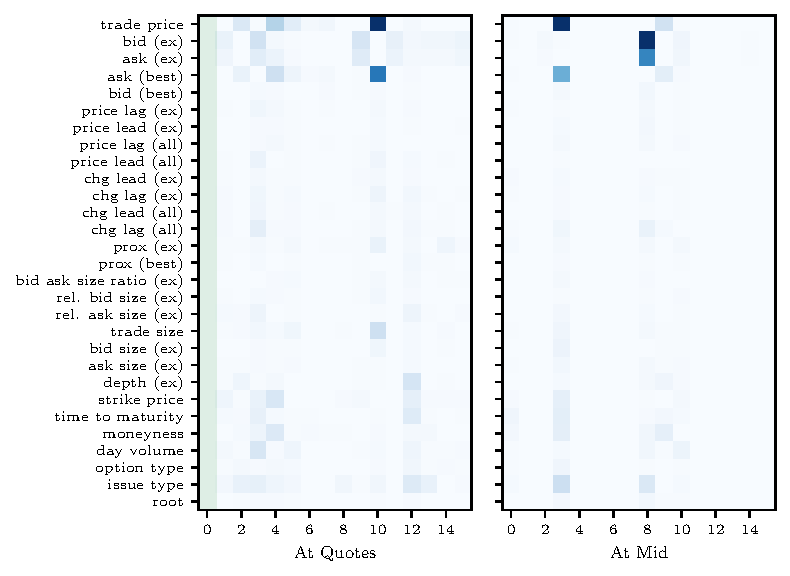
\includegraphics[width=1\textwidth]{attention_maps_ise_quotes_mid.pdf}
    \caption[Attention Maps of FT-Transformer]{Attention maps of FT-Transformer trained on \gls{ISE} data with \gls{FS} option. The left plot contains attention weights of \num{16} trades at the quotes and the right plot of \num{16} midspread trades. Each column represents a trade and each row represents a feature. The intensity of the pixel represents the importance. $\mathtt{[CLS]}$ token excluded, as suggested in \textcite[][4]{cheferGenericAttentionmodelExplainability2021}. The green area marks a trade, that was correctly classified by the network. Details on the trade are given below.}
    \label{fig:attention-maps-ise}
\end{figure}

Visually, the trade price and quotes at the exchange or inter-exchange level are important and frequently used. This aligns with theory, as these features are core to the quote rule and numerous hybrid algorithms. Also, quote-based algorithms are among the best performing in our dataset. Aside from the trade price, features required to estimate the tick rule attain only spurious attributions. Considering the devastating performance of tick-based algorithms in option trade classification, this is unsurprising. Features from the depth and trade size rule, such as the trade size, are used selectively for trades at the quotes. In this subset, option-specific features like the issue type, moneyness, time to maturity, or daily trading volume of the option series receive relatively high attention scores.  Overall, engineered features, like the proximity to quotes, attain low attention scores, which suggests that the Transformer itself can synthesize the feature from the \emph{raw} bid, ask, and trade price.

The model assigns higher attention scores to features present in rule-based algorithms. Due to the possible link to rule-based trade classification, it is worthwhile to explore, if the fine-grained patterns learned by specific attention heads translate to existing trade classification rules i.e., if specific tokens attend to features that are jointly used in rule-based classification. This information is sacrificed when aggregating over multiple attention heads and layers, as done for \cref{fig:attention-maps-ise}, but readily available from individual attention heads. To analyze this further, we adapt the approach of \textcite[][4]{clarkWhatDoesBERT2019} to our context and probe individual attention heads.

\begin{figure}[h!]
    \subfloat[Tick Rule-like Head (3,5)\label{fig:head-tick}]{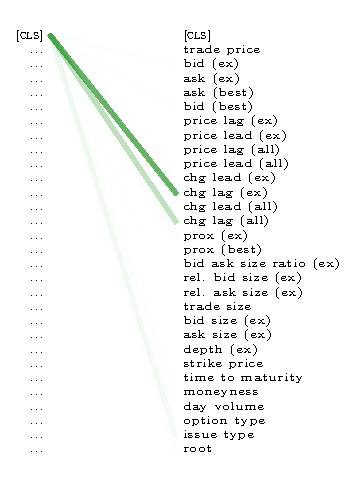
\includegraphics[width=0.3\textwidth]{attention_head_5_layer_3_color_green_ise_quotes_mid.pdf}}
    \hfill
    \subfloat[Trade Size Rule-like Head (3,8)\label{fig:head-tsize}]{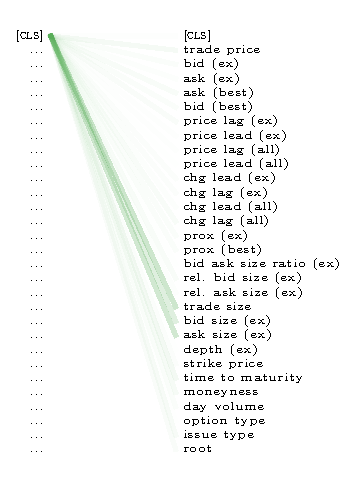
\includegraphics[width=0.3\textwidth]{attention_head_8_layer_3_color_green_ise_quotes_mid.pdf}}
    \hfill
    \subfloat[\glsentryshort{LR}-Like Head (4,8)\label{fig:head-lr}]{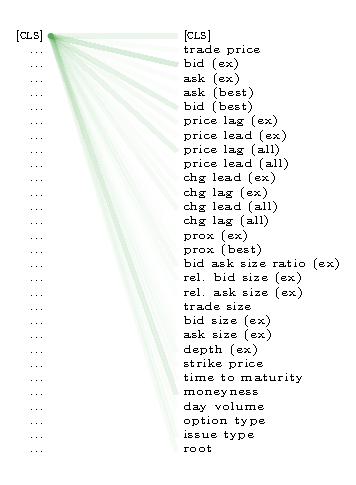
\includegraphics[width=0.3\textwidth]{attention_head_8_layer_4_color_green_ise_quotes_mid.pdf}}
    \caption[Rule-like Roles of Selected Attention Heads]{Attention heads that correspond to trade classification rules. Tuple denotes the location of the attention head in the model in the form of (layer, head). The intensity of the line represents the strength of attention weight. Attentions are only visualized for the $\mathtt{[CLS]}$ token. The model is trained on \gls{ISE} data. Visualizations based on code by \textcite[][4]{clarkWhatDoesBERT2019}.}
    \label{fig:rule-like-attention-heads}
\end{figure}

We study attention weights of one specific trade in detail, which is marked in green in \cref{fig:attention-maps-ise}. The trade has the following properties: trade price \SI{3.5}[\$]{}, trade size \SI{5}[]{} contracts, ask at exchange, \SI{3.85}[\$]{}, bid at exchange \SI{3.5}[\$]{}, ask size \SI{11}[]{} contracts, and bid size \SI{10}[]{} contracts, classified as sell. \cref{fig:rule-like-attention-heads} depicts the result for selected attention heads involved in classifying the specific trade. The remaining attention heads are visualized in \cref{app:attention-heads-of-transformer}. Each subplot depicts the features to which the classification token $\mathtt{[CLS]}$ attends too. The attention weight determines the intensity of the line between the two. 

Referring to the results from the appendix, we note that attention heads learn diverse patterns, as most heads attend to different tokens at once learning different relations. However, certain heads exhibit redundancy. For earlier layers in the network, the classification tokens gather from multiple tokens with uniform attention weights, whereas for the final self-attention layers, attention heads specialize in relations that seem related to rule-based trade classification. \cref{fig:head-tick} depicts a classification head that focuses solely on the change in trade price akin to the tick rule. In \cref{fig:head-tsize} the classification token in the neighboring head gathers simultaneously from multiple size-related features similar to the trade size rule. Finally, \cref{fig:head-lr} is alike to the \gls{LR} algorithm with additional dependencies on the moneyness. For other attention heads the purpose they serve in the network remains open. 

The redundancy between attention heads is possibly explained by the use of attention dropout in our networks (cp. \cref{sec:hyperparameter-tuning}), which randomly deactivates units of the network during training and forces the network to learn redundant representations. A similar point is made by \textcite[][8--9]{clarkWhatDoesBERT2019} for the related \gls{BERT} model. Our finding of uniform attention weights in earlier layers of the network is consistent with the of \textcite[][4]{abnarQuantifyingAttentionFlow2020} made for \gls{BERT}.

When repeated for other trades, the identified roles of the attention heads are partially retained, but it is important to highlight that a more comprehensive analysis is required. We suggest revisiting this topic in future research as it potentially enables uncovering new rule-based approaches and understanding Transformer-based trade classification in more detail.

\textbf{Embedding Visualization}

For the Transformer we know from \cref{sec:token-embeddings}, that embeddings can capture similarities by arranging related objects closer in embedding space. Visualizing the learned embeddings enables insights into the model.

The embeddings are queried from the feature tokenizer in FT-Transformer. The similarity between embeddings is measured by cosine distance in embedding space. The high-dimensional embeddings are then projected into 2D space using $t$-SNE \autocite[\checkmark][2587]{vandermaatenVisualizingDataUsing2008}. As straightforward to interpret, we focus our analysis on the root, but note, that it applies to any numerical and categorical embeddings.

\cref{fig:categorical-embeddings} illustrates the embeddings exemplary for SPDR S\&P 500 Trust ($\mathtt{SPY}$) and JPMorgan Chase \& Co ($\mathtt{JPM}$) which can be \emph{qualitatively} interpreted.\footnote{As our analysis is condensed to two randomly chosen examples, we encourage the reader to use our interactive visualization for further exploration. Accessible here \url{https://projector.tensorflow.org/?config=https://raw.githubusercontent.com/KarelZe/Embeddings/main/embedding_projector.config.json}.}

\begin{figure}[h!]
    \subfloat[Most Similar Embeddings to $\mathtt{SPY}$\label{fig:cat-embeddings-spy}]{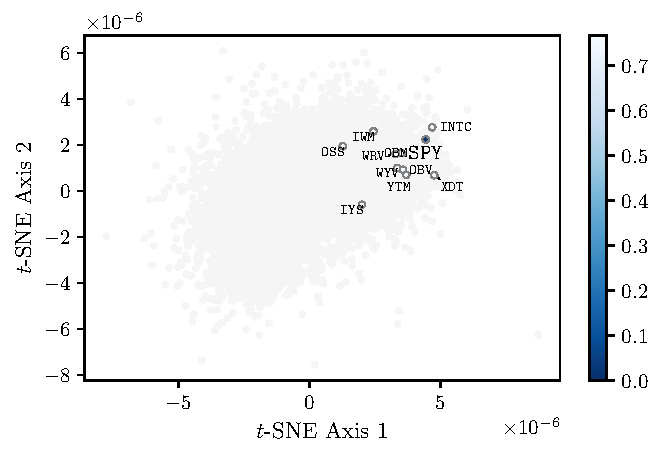
\includegraphics[width=0.6\textwidth]{categorical_embeddings_SPY.pdf}}
    \vfill
    \subfloat[Most Similar Embeddings to $\mathtt{JPM}$\label{fig:cat-embeddings-jpm}]{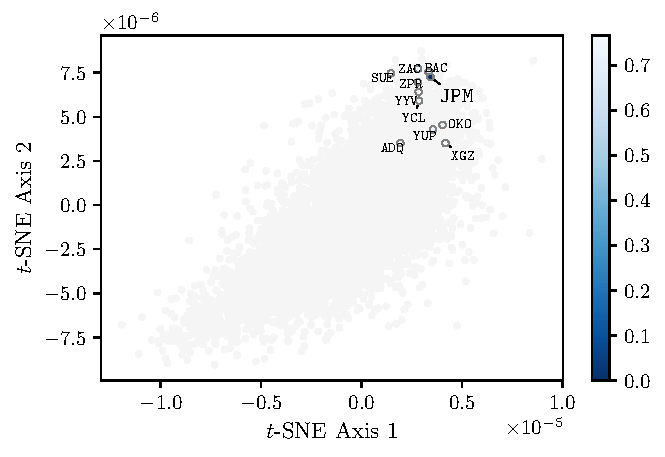
\includegraphics[width=0.6\textwidth]{categorical_embeddings_JPM.pdf}}
    \caption[Embeddings of Selected Underlyings]{Embeddings of selected underlyings. The plot depicts the projected embedding of SPDR S\&P 500 ETF ($\mathtt{SPY}$) and JPMorgan Chase \& Co ($\mathtt{JPM}$) and their most similar embeddings. Embeddings are projected into 2D space using $t$-SNE. The ten most similar embeddings by cosine distance in the original space are colored and annotated. The model is trained on \gls{ISE} data.}
    \label{fig:categorical-embeddings}
\end{figure}

For SPDR S\&P 500 ETF ($\mathtt{SPY}$) in \cref{fig:cat-embeddings-spy}, similar embeddings include iShares Russell 2000 ($\mathtt{IWM}$), iShares Russel 2000 ($\mathtt{WYV}$), SPDR S\&P 500 ETF ($\mathtt{OBV}$), and Direxion shares ETF ($\mathtt{XDT}$). This aligns with the intuition that \glspl{ETF} track identical or related indices. The model distinguishes \glspl{ETF} from other securities based on the feature issue type. Additional similar embeddings consist of Citigroup Inc. ($\mathtt{WRV}$), Kohl's Corp. ($\mathtt{OSS}$), Google Inc. ($\mathtt{YTM}$), and Intel Corp. ($\mathtt{INTC}$), which are long-term index constituents.

Regarding JPMorgan Chase \& Co. ($\mathtt{JPM}$) in \cref{fig:cat-embeddings-jpm}, the most similar embedding is the of Bank of America ($\mathtt{BAC}$). Other similar embeddings include financial service providers like Amerigroup ($\mathtt{XGZ}$) and Janus Henderson Group ($\mathtt{ZPR}$). These results suggest that the model learned to group US financials, even without sector information provided. However, this argumentation does not apply to other related embeddings such as the Apollo Group ($\mathtt{OKO}$) or United Parcel Service of America ($\mathtt{YUP}$). % Autodesk Inc. ($\mathtt{ADQ}$) , Centex Corp. ($\mathtt{YYV}$), United Parcel Service of America ($\mathtt{YUP}$), Wild Oats Markets ($\mathtt{ZAC}$), SPDR S\&P 500 ETF ($\mathtt{SUE}$), and SPDR Dow Jones Industrial Average ($\mathtt{DIA}$).

While these exemplary results indicate that the model can learn meaningful representations of the underlying, we must acknowledge its limitations. Both underlyings are frequently traded in our dataset, which may lead to meaningful embeddings. For infrequent underlyings, embeddings are likely to be close to their random initialization and lack meaningful patterns due to limited parameter updates and missing context. This issue is analogous to handling rare vocabulary items found in natural language processing. As the underlying plays a subordinate role in classification, this caveat is accepted.

\textbf{SAGE Values}

We compare the feature importances of rule-based and machine learning-based classifiers using \gls{SAGE}, which offers a clear interpretation of each feature's contribution to the prediction. The zero-one loss is chosen as a loss function, which is appealing due to the direct link to accuracy. Based on the distribution of the \gls{ISE} test set, a na\"ive prediction of the majority class yields an accuracy of \SI{51.4027}{\percent} or a zero-one loss of $1- \num{0.514027} = \num{0.485973}$. \gls{SAGE} attributes the outperformance of machine learning or rule-based classifiers over the na\"ive prediction to the features based on Shapley values. The sum of all \gls{SAGE} values for a given predictor represents the difference in loss compared to the na\"ive classification.

\begin{figure}[h!]
    \centering
    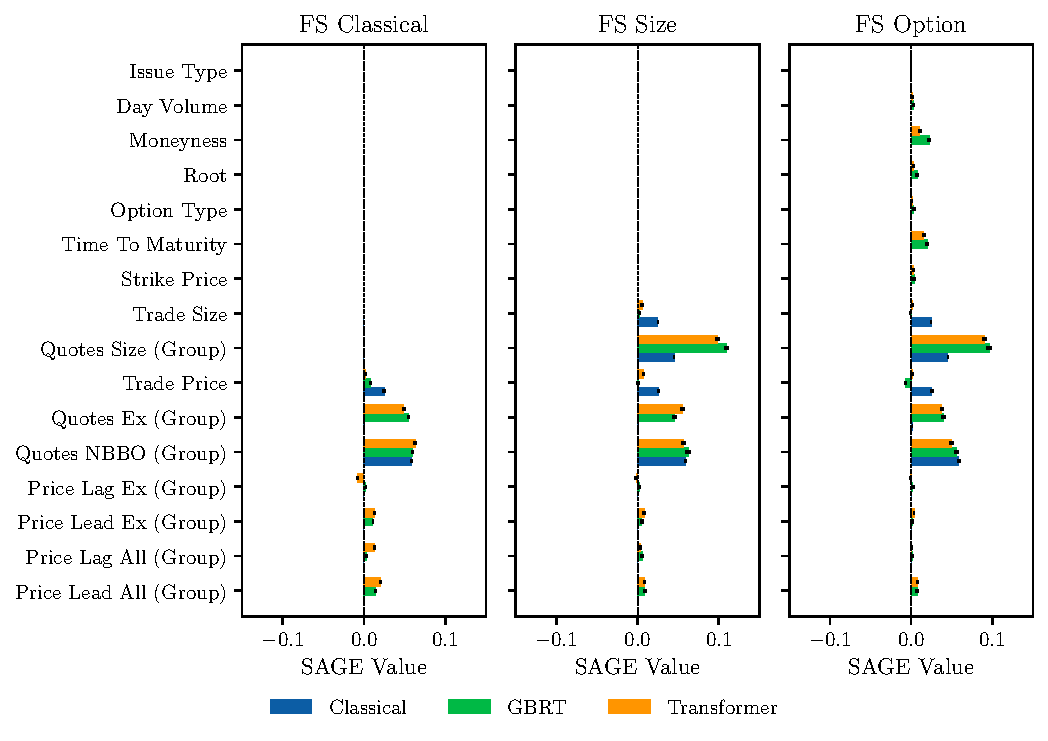
\includegraphics[width=1\textwidth]{sage-importances.pdf}
    \caption[\glsentryshort{SAGE} Feature Importances For Classifiers]{\gls{SAGE} feature importances of rule-based and machine learning-based classifiers.}
    \label{fig:sage-importances}
\end{figure}

From \cref{fig:sage-importances} that all models achieve the largest improvement in loss from quoted prices and if provided from the quoted sizes. The contribution of the \gls{NBBO} to performance is roughly equal for all models, suggesting that even simple heuristics effectively exploit the data. For machine learning-based predictors, quotes at the exchange level hold equal importance in classification. This contrast with \gls{GSU} methods, which rely less on exchange-level quotes and mostly classify trades based on upstream rules. The performance improvements from the trade size and quoted size, are slightly lower for rule-based methods compared to machine learning-based methods.  Transformers and \glspl{GBRT} gain performance from the addition of option features, i.e., moneyness and time-to-maturity. In conjunction with the results from the robustness checks, this suggests that the improvements observed for long-running options or \gls{ITM} options are directly linked to the moneyness or time to maturity of the traded option itself. However, it remains unclear how these features interact with others. Regardless of the method used, changes in trade price before or after the trade are irrelevant for classification and can even harm performance. Similarly, additional features such as option type, issue type, the trading volume of the option series, and the underlying are also irrelevant. Thus, we note that there is a significant overlap between the importance of features in classical trade classification rules and machine learning-based predictors.

\todo{Importance of Moneyness and Time-to-Maturity. How do these results fit into a broader picture?}
\todo{Distribution in Sample: TTM, Trade Size, Moneyness}

\clearpage

\section{Application in Transaction Cost Estimation}\label{sec:application}

\textbf{Preliminaries}

Albeit the classification accuracy is a reasonable measure for comparing classifiers, one cannot immediately infer how changes in accuracy e.~g., an improvement by \SI{1}{\percent}, affect the application domains. In an attempt to make our results tangible, we apply all algorithms to estimate trading cost, a problem we previously identified to be reliant on correct trade classification (cp. \cref{sec:introduction}) and a common testing ground for trade classification rules \autocites[cp.][540--541]{ellisAccuracyTradeClassification2000}[\checkmark][569--570]{finucaneDirectTestMethods2000}[\checkmark][271--278]{petersonEvaluationBiasesExecution2003}[\checkmark][896--897]{savickasInferringDirectionOption2003}.

One of the most widely adopted measures for trading costs is the effective spread \autocite[\checkmark][112]{Piwowar_2006}. It is defined as the difference between the trade price and the fundamental value of the asset \autocite[\checkmark][238--239]{bessembinderIssuesAssessingTrade2003}. Following \textcite[\checkmark][238--239]{bessembinderIssuesAssessingTrade2003}, we define the \emph{nominal, effective spread} as
\begin{equation}
    S_{i,t} = 2 (P_{i,t} - V_{i,t}) D_{i,t}.
    \label{eq:effective-spread}
\end{equation}

Like before, $i$ indexes the security and $t$ the point in time. Here, $D_{i,t}$ is the trade direction, which is either $1$ for customer buy orders and $-1$ for sell orders. If the trade initiator is known, we set $D_{i,t} = y_{i,t}$ and $D_{i,t}=\hat{y}_{it}$, if inferred from a rule or classifier. As the fundamental value $V_{i,t}$ is unobserved at the time of the trade, we follow a common track in research and use the midpoint of the prevailing quotes as an observable proxy.\footnote{An alternative treatment for options is discussed in \textcite[\checkmark][4975--4976]{muravyevOptionsTradingCosts2020} Our focus is on the midspread, as it is the most common proxy for the value.} This is also a natural choice, under the assumption that, on average, the spread is symmetric and centered around the true fundamental value \autocite[\checkmark][1018]{leeMarketIntegrationPrice1993}. We multiply the so-obtained half-spread by $2 \times$ to obtain the effective spread, which represents the cost for a round trip trade involving a buy and sell excluding commissions.

Apparent from \cref{eq:effective-spread}, poor estimates for the predicted trade direction, lead to an under or overestimated effective spread, and hence to a skewed trade cost estimate. Only for trades at the midspread, the predicted trade direction is irrelevant, since the effective spread is zero. By comparing the true effective spread from the estimated, we can derive the economic significance. A classifier correctly classifying every trade, achieves an effective spread estimate equal to the true spread. For a random classifier, the effective spread is around zero, as misclassification estimates the spread with the opposite sign, which offsets with correct, random estimates for other trades.

For convenience, we also calculate the \emph{relative effective spread} as
\begin{equation}
    {PS}_{i,t} = S_{i,t} / V_{i,t}.
\end{equation}

Adapted from \textcite[\checkmark][158]{theissenTestAccuracyLee2001} a Wilcoxon test is conducted to assess if the medians of the estimated, effective spread and the true effective spread are equal.

\textbf{Results}

The true and the estimated effective spreads for the test sets are shown in the \cref{tab:effective-spread} aggregated by mean. \textcite[\checkmark][896--897]{savickasInferringDirectionOption2003} estimated the effective spreads of rules on an older subset of option trades at the \gls{CBOE}, which can be compared against. Our results match theirs in magnitude.

\begin{table}[!ht]
    \centering
    \begin{threeparttable}
    \sisetup{
        round-precision = 3, 
      }
    \begin{tabular}{llSSSS}
        \toprule
        {}                                               & {}   & \multicolumn{2}{c}{\gls{ISE}} & \multicolumn{2}{c}{\gls{CBOE}}                                 \\ \cmidrule(lr){3-4}\cmidrule(lr){5-6}
        {Classifier}                                     & {FS} & {Dollar}                      & {Relative}                     & {Dollar} & {Relative}         \\ \midrule
        \multicolumn{6}{l}{Rule-Based}                                                                                                                           \\
        \tabindent $\operatorname{tick}_{\mathrm{ex}}$   & 1    & 0.015534                      & 0.010777 \tnote{*}             & 0.014179 & 0.022880 \tnote{*} \\
        \tabindent $\operatorname{quote}_{\mathrm{ex}}$  & 1    & 0.163333                      & 0.162074 \tnote{*}             & 0.125388 & 0.142093 \tnote{*} \\
        \tabindent $\operatorname{lr}_{\mathrm{ex}}$     & 1    & 0.163333                      & 0.162074 \tnote{*}             & 0.125388 & 0.142093 \tnote{*} \\
        \tabindent $\operatorname{emo}_{\mathrm{ex}}$    & 1    & 0.046443                      & 0.084442 \tnote{*}             & 0.041138 & 0.074176 \tnote{*} \\ 
        \tabindent $\operatorname{clnv}_{\mathrm{ex}}$   & 1    & 0.116247                      & 0.132842 \tnote{*}             & 0.086715 & 0.110510 \tnote{*} \\ 
        \tabindent $\operatorname{gsu}_{\mathrm{small}}$ & 2    & 0.065670                      & 0.096277 \tnote{*}             & 0.084145 & 0.107195 \tnote{*} \\
        \tabindent $\operatorname{gsu}_{\mathrm{large}}$ & 2    & 0.016734                      & 0.044854 \tnote{*}             & 0.053114 & 0.072212 \tnote{*} \\ \midrule
        \multicolumn{6}{l}{Supervised}                                                                                                                           \\
        \tabindent \gls{GBRT}                            & 1    & 0.074294                      & 0.091619 \tnote{*}             & 0.060933 & 0.095318 \tnote{*} \\
        \tabindent \gls{GBRT}                            & 2    & 0.042556                      & 0.069838 \tnote{*}             & 0.036213 & 0.071433 \tnote{*} \\
        \tabindent \gls{GBRT}                            & 3    & 0.039437                      & 0.066473 \tnote{*}             & 0.034674 & 0.066758 \tnote{*} \\ 
        \tabindent  FT-Transformer                       & 2    & 0.030291                      & 0.065596 \tnote{*}             & 0.024942 & 0.063574 \tnote{*} \\
        \tabindent  FT-Transformer                       & 1    & 0.065871                      & 0.086339 \tnote{*}             & 0.057153 & 0.090205 \tnote{*} \\
        \tabindent  FT-Transformer                       & 3    & 0.029874                      & 0.063486 \tnote{*}             & 0.021487 & 0.057358 \tnote{*} \\ \midrule
        \multicolumn{6}{l}{Semi-Supervised}                                                                                                                      \\
        \tabindent \gls{GBRT}                            & 1    & 0.075724                      & 0.092439 \tnote{*}             & 0.065420 & 0.096814 \tnote{*} \\
        \tabindent \gls{GBRT}                            & 2    & 0.043359                      & 0.072062 \tnote{*}             & 0.039600 & 0.073760 \tnote{*} \\
        \tabindent \gls{GBRT}                            & 3    & 0.043240                      & 0.069230 \tnote{*}             & 0.037083 & 0.067946 \tnote{*} \\ 
        \tabindent  FT-Transformer                       & 1    &                               & \tnote{*}                      &          & \tnote{*}          \\
        \tabindent  FT-Transformer                       & 2    &                               & \tnote{*}                      &          & \tnote{*}          \\
        \tabindent  FT-Transformer                       & 3    &                               & \tnote{*}                      &          & \tnote{*}          \\ \midrule
        True Effective Spread                            &      & 0.004926                      & 0.037159                       & 0.012219 & 0.025122           \\ \bottomrule
        % Quoted Spread                                    &      &                                                   &                                                    &          &                 \\ \bottomrule
    \end{tabular}
    \begin{tablenotes}\footnotesize
        \item[*] $p \leq 0.01$.
    \end{tablenotes}
\end{threeparttable}
    \caption[Effective Spreads Estimates]{Effective spreads estimates of trade classification rules and classifiers. Results are calculated on \gls{ISE} and \gls{CBOE} test set and averaged over all trades within the samples. Classifiers match the configuration of \cref{sec:hyperparameter-tuning}.}
    \label{tab:effective-spread}
\end{table}

In summary, quote-based algorithms like the quote rule and the \gls{LR} algorithm severely overestimate the effective spread. The overestimate is less severe for the \gls{CLNV} algorithm due to stronger dependency on the tick rule. The tick rule itself achieves estimates closest to the true effective spread, which is \num[round-mode=places, round-precision=3]{0.004926}[\$]{} and \num[round-mode=places, round-precision=3]{0.012219}[\$]{} for the \gls{ISE} and \gls{CBOE} sample respectively. As primarily tick-based algorithms, like the tick rule or \gls{EMO} rule, act as a random classifier in our samples, we conclude that the close estimate is an artifact of randomness, not due to superior predictive power. This observation is in line with \textcite[\checkmark][897]{savickasInferringDirectionOption2003}, who make a similar argument for the \gls{EMO} rule on \gls{CBOE} trades. For rule-based algorithms $\operatorname{gsu}_{\mathrm{large}}$ provides reasonable estimates of the effective spread while achieving high classification accuracy.

From our supervised classifiers the FT-Transformer or \gls{GBRT} trained on \gls{FS} option provides estimates closest to the true effective spread, in particular on the \gls{CBOE} sample. For semi-supervised classifiers, Transformer-based models approximate the true effective spread best. This best manifests in a predicted effective spread at the \gls{ISE} of \SI[round-mode=places, round-precision=3]{0.013118}[\$]{} versus \SI[round-mode=places, round-precision=3]{0.004926}[\$]{}. The null hypothesis of equal medians is rejected at the \SI{1}{\percent} level for all classifiers.

Thus, \gls{GSU} method (large) provides the best estimate of the effective spread if the true labels are absent. For labeled data, Transformer or gradient boosting-based approaches can provide more accurate estimates. The de facto standard, the \gls{LR} algorithm, fails to deliver accurate estimates and may bias research.

\todo{“In addition, my results offer little help in answering why option bid-ask spreads are so large. This is one of the biggest puzzles in the options literature—existing theories of the option spread fail to explain its magnitude and shape (Muravyev and Pearson (2014)).”}
\todo{compare against \textcite[][4981]{muravyevOptionsTradingCosts2020} or \autocite{kaeckPriceImpactBid2022}}
\todo{Think about reporting as a percentage. Adjust the formula from above.}
\todo{Look into \textcite{muravyevOptionsTradingCosts2020}}
\todo{Options listed on multiple exchanges have narrower spreads than those listed on a single exchange, but the difference diminishes as option volume increases. Option spreads become wider when a competing exchange delists the option.\autocite{mayhewCompetitionMarketStructure2002}}
